\documentclass{article}
\usepackage{listings}

\usepackage{amsmath}
\usepackage{amsfonts}
\usepackage[hidelinks]{hyperref}
\usepackage{xcolor}
  \renewcommand\UrlFont{\color{blue}}

\usepackage{cleveref}
\usepackage{graphicx}
\usepackage{subcaption}
\usepackage{float}
\usepackage{diagbox}
\usepackage{physics}
\usepackage{mathtools}
\usepackage{braket}
\usepackage{booktabs}

\usepackage{algorithm}
\usepackage{algpseudocode}
  \renewcommand{\algorithmicrequire}{\textbf{Input:}}
  \renewcommand{\algorithmicensure}{\textbf{MCMC Input:}}

\usepackage{tikz}
  \usetikzlibrary{backgrounds,fit,positioning,calc,graphs}
  \pgfdeclarelayer{background}
  \pgfdeclarelayer{backbackground}
  \pgfsetlayers{backbackground,background,main}
  \tikzset{
      framed,
      node distance=3mm,
      layer/.style={rectangle, draw=black, font=\fontsize{6}{6}\selectfont, fill=cyan!30, minimum size=4mm},
      sum/.style={circle, draw=black, font=\fontsize{6}{6}\selectfont, fill=red!30, inner sep=1pt, minimum size=4mm},
      annot/.style={font=\fontsize{6}{6}\selectfont},
      bkg/.style={draw, dotted, fill=green!30}
  }

\usepackage{stackengine}
\usepackage{courier}

\DeclareMathOperator*{\argmax}{arg\,max}
\DeclareMathOperator*{\argsup}{arg\,sup}

\makeatletter
\newcount\my@repeat@count
\newcommand{\myrepeat}[2]{%
  \begingroup
  \my@repeat@count=\z@
  \@whilenum\my@repeat@count<#1\do{#2\advance\my@repeat@count\@ne}%
  \endgroup
}
\makeatother

\renewcommand{\figurename}{Supplementary Figure}
\crefname{figure}{Supplementary Figure}{Supplementary Figures}
\renewcommand{\tablename}{Supplementary Table}
\crefname{table}{Supplementary Table}{Supplementary Tables}
\crefname{algorithm}{Algorithm}{Algorithms}

\title{CRISPR AI}

\author{
    Shi, Xin\\
    \texttt{shixinsk@163.com}
    \and
    Li, Chenyu\\
    \texttt{951899997@qq.com}
    \and
    Li, Jingwei\\
    \texttt{ljw2017@sjtu.edu.cn}
    \and
    Wu, Qiang\\
    \texttt{qiangwu@sjtu.edu.cn}}

\date{\today}

\pagenumbering{gobble}

\begin{document}

\maketitle

% \tableofcontents

\section{The workflow of naapam}
\label{sec:naapam}

The overall workflow to correct the editing profile of CRISPR/Cas9 system is shown in \cref{fig:workflow}. We describe the steps in detail in the subsections below.

\begin{figure}[H]
  \centering
  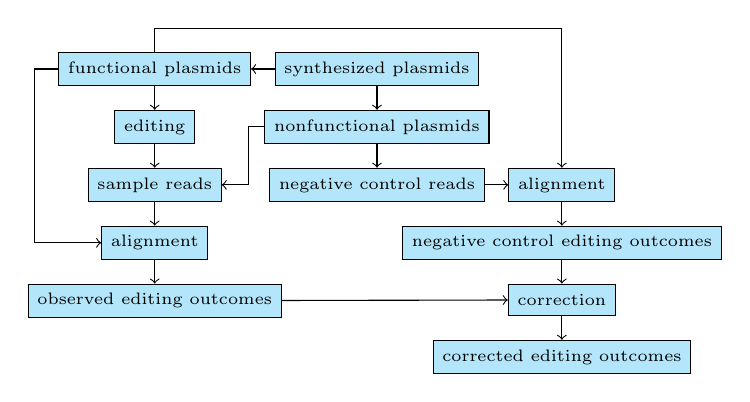
\begin{tikzpicture}
    \node[layer] (SP) {synthesized plasmids};
    \node[layer, below=of SP] (NFP) {nonfunctional plasmids};
    \node[layer, below=of NFP] (NCR) {negative control reads};
    \node[layer, right=of NCR] (ALG2) {alignment};
    \node[layer, below=of ALG2] (NCEO) {negative control editing outcomes};
    \node[layer, below=of NCEO] (CORRECT) {correction};
    \node[layer, below=of CORRECT] (CEO) {corrected editing outcomes};
    \graph {
      (SP) -> (NFP) -> (NCR) -> (ALG2) -> (NCEO) -> (CORRECT) -> (CEO);
    };

    \node[layer, left=of SP] (FP) {functional plasmids};
    \node[layer, below=of FP] (EDIT) {editing};
    \node[layer, below=of EDIT] (SR) {sample reads};
    \node[layer, below=of SR] (ALG1) {alignment};
    \node[layer, below=of ALG1] (OEO) {observed editing outcomes};
    \graph {
      (SP) -> (FP) -> (EDIT) -> (SR) -> (ALG1) -> (OEO) -> (CORRECT);
    };

    \draw[->] (FP) -- ($(FP.west) + (-3mm,0)$) |- (ALG1);
    \draw[->] (NFP) -- ($(NFP.west) + (-2mm,0)$) |- (SR);
    \draw[->] (FP) -- ($(FP.north) + (0,3mm)$) -| (ALG2);
  \end{tikzpicture}
  \caption{The overall workflow to correct the editing profile.}\label{fig:workflow}
\end{figure}

\subsection{Parse the sample reads}

The raw sequencing files contain duplicates of the same read. We extract non-duplicated read pairs and reserve the pair counts. Then we parse the elements from the read pairs based on the plasmid design (\cref{fig:plasmid_design}). In detail, the plasmid consists of R1 barcode, the last 19 bps of U6 (R1 primer), G, sgRNA, scaffold, G, 44bp target sequence, CAG, plasmid barcode, 20bp R2 primer and R2 barcode. R1 sequences the plasmid from U6. R2 sequences the reverse-complement of the plasmid. Both R1 and R2 are prefixed by sequencing barcode. Because primer and scaffold are fixed across all plasmids, we first extract primer and scaffold from R1 and R2. By using the alignment library of biopython, we allow small mutations in primer and scaffold. For R1, the segment between primer and scaffold is sgRNA. For R2, that is barcode + CTG + target sequence.
\begin{figure}[H]
  \centering
  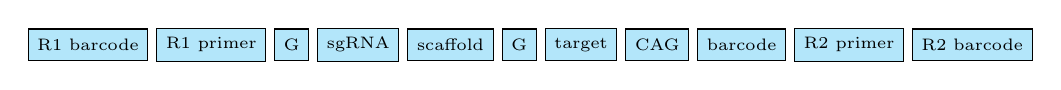
\begin{tikzpicture}[node distance=1mm]
    \node[layer] (R1B) {R1 barcode};
    \node[layer, right=of R1B] (R1P) {R1 primer};
    \node[layer, right=of R1P] (TSS) {G};
    \node[layer, right=of TSS] (SG) {sgRNA};
    \node[layer, right=of SG] (SC) {scaffold};
    \node[layer, right=of SC] (TES) {G};
    \node[layer, right=of TES] (T) {target};
    \node[layer, right=of T] (CAG) {CAG};
    \node[layer, right=of CAG] (BC) {barcode};
    \node[layer, right=of BC] (R2P) {R2 primer};
    \node[layer, right=of R2P] (R2B) {R2 barcode};
  \end{tikzpicture}
  \caption{The design of plasmid.}\label{fig:plasmid_design}
\end{figure}

To parse the plasmid barcode in R2, we build bowtie2 index for each plasmid barcode. Then we map the R2 segment between primer and scaffold ({\it i.e.} barcode + CTG + target sequence) to the plasmid barcodes. Finally, We extract the matching information, including the map score in AS tag, the id of the matched barcode, and the position of the matching.

We use a similar method to parse the sgRNA in R1 and the protospacer sequence in R2. In detail, we build bowtie2 index for each sgRNA sequence. Then we map sgRNA in R1 and target sequence in R2 to the sgRNA sequences. Finally, we extract the matching information, including the map score in AS tag, the id of the matched sgRNA sequence, and the position of the matching.

\subsection{Get the editing targets}

Using the designed plasmids as the editing targets is not accurate because the synthesis of the plasmids is error-prone. Thus, the actual plasmid transferred into the cells may be quite different from the design. Instead, we collect the editing targets from the control samples (samples without Cas9). We group the control samples by the synthesis libraries, remove duplicates and reserve the counts. These control reads are candidates of editing targets. We filter control reads containing out-of-distribution values of the following criteria.
\begin{itemize}
  \item Abnormally short or long component length.
  \item Low alignment score to the designed sequence (e.g. low quality primer, barcode, spacer and scaffold).
  \item U6 flags necessary for transcription (two Gs padding the sgRNA and scaffold).
  \item Low count across all control samples.
  \item Reads without matched barcode/protospacer or with inconsistent barcode and protospacer.
\end{itemize}

Even after removing duplicates and filtering out low quality control reads, the diversity of the control reads is still too large as editing targets. To further decrease the control read diversity, we align control reads to the designed plasmids to get the synthesis type of each read, and cluster control reads by synthesis types. In detail, we neglect irrelevant small synthesis errors away from the cleavage site and only classify control reads by the main synthesis error around the cleavage site, including resections and templated insertions at both ends and the random insertions. We then apply the quality control over the synthesis types. Firstly, we apply a plasmid barcode-wise filtering. We filter out all synthesis types refer to the designed plasmid of a barcode if the plasmid barcode satisfies any of the following conditions.
\begin{itemize}
  \item Too many synthesis types.
  \item With both low total read count and low wild-type frequency.
  \item The second most common synthesis type is too abundant compared with the most common synthesis type.
\end{itemize}
Secondly, we filter out synthesis types satisfying any of the following conditions.
\begin{itemize}
  \item Among all synthesis types of the plasmid of the barcode, the aggregated percentage of those less common than the current synthesis type is low.
  \item Among all synthesis types of the plasmid of the barcode, the rank of the synthesis type from the most common to the least common is high.
  \item The upstream or downstream deletion size is too large.
  \item The random insertion size is too large.
  \item The count of the synthesis type is too small.
\end{itemize}

We use the synthesis types passing filtering as editing targets. We align the sequencing reads in treatment samples to these targets instead of the designed plasmids to get the editing outcomes.


\subsection{The quality control of the sample reads}

We apply a quality control to the sample (both treatment with Cas9 and control without Cas9) reads before aligning them to the editing targets obtained by the previous step. We choose a loose criteria because it is expected that treatment reads will contain more mutants due to the CRISPR/Cas9 editings. In detail, we filter out the sample reads with out-of-distribution values for any of the following criteria.
\begin{itemize}
  \item Abnormally short or long lengths for R1/R2 primer or scaffold spacer.
  \item Low alignment score to the designed sequence for R1/R2 primer, scaffold or protospacer.
  \item The U6 flag necessary for transcription start (the G padding the sgRNA).
  \item Low count across all samples.
  \item Reads without matched barcode/protospacer or with inconsistent barcode and protospacer.
\end{itemize}

\subsection{Align the sample reads to the editing targets}

We then assign the sample reads to the editing targets collected from the control samples based on the matched plasmid barcodes. To analyze indels, especially the templated insertions in high accuracies, we align the sample read to the editing target by the bioconda package rearr (version 1.0.11). If a sample read is assigned to a plasmid barcode with multiple editing targets, we align it to each of the editing target and distribute the count of the sample read to each editing target as follows.
\begin{itemize}
  \item Normalize the count of the editing target to get the priori distribution for the count of the sample read.
  \item Normalize the alignment score between the sample read and the editing target by a temperature and use softmax to calculate the conditional probability.
  \item By Bayes' theorem, we can get the posteriori distribution of the count of the sample read from the priori distribution and the conditional probability.
\end{itemize}
We collect the alignment results and apply a read-wise filter based on the alignment score. We then aggregate all reads based on the editing outcome near the cleavage site predicted by rearr.

\subsection{Filter out the editing target}

During the analyses of the indels of the editing outcomes, we find that 1bp templated insertion is highly biased to 2bp upstream deletion, 2bp templated insertion is highly biased to 3bp upstream deletion, 3bp templated insertion is highly biased to 4bp upstream deletion and so on. After careful trouble shooting, we find that this is caused by the 1bp deletion synthetic error upstream to the cleavage site. An example of the 3bp templated insertion together with the 4bp upstream deletion caused by the 1bp deletion synthetic error is shown in \cref{fig:artifact_tem}.
\begin{figure}[H]
  \centering
  \begin{tabular}{l}
    \stackanchor[1pt]{
        \texttt{CTGGCAAACCACTTATGCTGCTGCT\clap{\textbf{|}}TCATAAATTTCCAGAATTCTGGCAA}
      }{
        \stackanchor[1pt]{
          \texttt{CTGGCAAACCACTTATGCTGC~~~~~~~~~~~~~~~~~~~~~~~~~~~~~}
        }{
          \texttt{~~~~~~~~~~~~~~~~~~~~~~GCTTCATAAATTTCCAGAATTCTGGCAA}
        }
      } \\
  \end{tabular}
  \caption{The 1bp deletion synthetic error make the artifact of the 3bp templated insertion together with the 4bp upstream deletion.}\label{fig:artifact_tem}
\end{figure}

Because long templated insertion is quite rare, even a low the synthesis error rate of the 1bp deletion upstream to the cleavage site in the editing target will lead to a great overestimate of the templated insertion rate. To remove these artifacts, we count the reads in all samples for each upstream deletion size (not necessarily happening templated insertions) and calculate their relative abundances to the upstream blunt end. We find that the relative abundance decreases exponentially with the upstream deletion size. Thus, we fit a linear model between the log of the relative abundance and the upstream deletion size, as shown in \cref{fig:relabun}.
\begin{figure}[H]
  \centering
  \includegraphics[width=0.5\textwidth]{/home/ljw/sdb1/naapam/figures/analyze/fit_ref/ci.pdf}
  \caption{The log of the relative abundance decrease linearly with the upstream deletion size.}\label{fig:relabun}
\end{figure}

We calculate the upper bound of the 95\% prediction interval as the upper limit of the relative abundance to the upstream blunt end for each upstream deletion size. We expect that these upper limits are good estimates for the relative upstream deletion abundance restricted to any given templated insertion size. We then filter out the editing targets with abnormally high abundance of any upstream deletion size restricted to any templated insertion size. We also filter out the editing targets with low total read count or low wild-type frequencies. For the editing targets passing the above criteria, we further filter out their editing outcomes as follows.
\begin{itemize}
  \item The upstream or downstream deletion size is too large.
  \item The random insertion size is too large.
  \item The ratio among all editing outcomes of the editing target is too high.
\end{itemize}

\subsection{Correct the mutant frequency by control sample}

Finally, we apply the correction method in previous works \cite{kim_prediction_2020,kim_high-throughput_2020}. For each editing target, we calculate its expected abundance in the treatment sample according to its abundance in the control sample. The observed abundance of editing target will be lower than expected because of the CRISPR/Cas9 editing on it. The editing outcomes mix with the nonfunctional plasmids. Thus, for each type of the editing outcomes, we estimate its expected abundance from the nonfunctional plasmids based on its abundance in the control sample, and subtract the result from the observed abundance. The negative subtraction results are corrected to zero.

\section{Model architecture selection}

We attempt models of various architectures, including the diffusion model (CRIfuser) \cite{campbell2022continuous,zhao2024unified}, transformer (CRIformer) \cite{su2024roformer}, long short-term memory (LSTM), convolutional neural network (CNN), multilayer perceptron (MLP), ridge regression and XGBoost, to predict the CRISPR editing profiles including deletion up to 25bp and templated insertion up to 6bp on each side of the cleavage site. We train each model on all the three datasets of the G-rich editor SpyCas9, A-rich editor SpyMac and optimized A-rich editor iSpyMac. We find that the diffusion model (CRIfuser) performances the best almost uniformly across all datasets and metrics (Extended Data Fig. 10a-c and \cref{fig:archi_select}a-c). The only exception is the mean square error for SpyMac dataset, where CRIfuser performs slightly worse than CRIformer (basically the same).
\begin{figure}[H]
  \centering
  \begin{subfigure}{0.5\textwidth}
    \includegraphics[width=\textwidth]{../benchmark/SX_spcas9_GreatestCommonCrossEntropy_select.pdf}
    \caption{Cross entropy loss for various model architectures trained on SpyCas9 dataset.}
  \end{subfigure}
  \begin{subfigure}{0.5\textwidth}
    \includegraphics[width=\textwidth]{../benchmark/SX_spymac_GreatestCommonCrossEntropy_select.pdf}
    \caption{Cross entropy loss for various model architectures trained on SpyMac dataset.}
  \end{subfigure}
  \begin{subfigure}{0.5\textwidth}
    \includegraphics[width=\textwidth]{../benchmark/SX_ispymac_GreatestCommonCrossEntropy_select.pdf}
    \caption{Cross entropy loss for various model architectures trained on iSpyMac dataset.}
  \end{subfigure}
  \caption{Metrics for model architecture selection.}\label{fig:archi_select}
\end{figure}

\section{Benchmark with models in previous works}

Previous works have tried to solve the problem of predicting the CRISPR editing profile from the sgRNA, including inDelphi \cite{shen2018predictable}, FOREcasT\cite{allen2019predicting} and Lindel \cite{chen2019massively}. We list their methods in \cref{tab:previous_works}.
\begin{table}[H]
    \centering
    \begin{tabular}{|l|l|}
        \hline
        name & method \\
        \hline
        inDelphi\cite{shen2018predictable} & multilayer perceptron \\
        Lindel\cite{chen2019massively} & logistic regression \\
        FOREcasT\cite{allen2019predicting} & logistic regression \\
        \hline
    \end{tabular}
    \caption{Tools of previous works and their methods.}\label{tab:previous_works}
\end{table}
To compare CRIfuser with inDelphi, FOREcasT and Lindel, we train them on the same datasets as CRIfuser. We conduct the same comparison as in the selection of model architectures. CRIfuser performs uniformly better than models in previous works in all datasets and metrics (Fig. 6b-d and Extended Data Fig. 10d-f).

\section{Shapley additive explanation}

We use SHAP (shapley additive explanation) to explain the model prediction for small indels (indels for both ends of DSB are less than or equal to 2bp), large indels (strictly more than 2bp indels for both ends of DSB), unilateral (one end of DSB has an indel less than or equal to 2bp, and the other has one strictly more than 2bp) and MMEJ (large deletions caused by MMEJ). \cref{fig:shap_selection} shows the SHAP results for models in the selection of model architectures.
\begin{figure}[H]
  \centering
  \begin{subfigure}{0.24\linewidth}
    \includegraphics[width=\linewidth]{../summary_shap/SX_spcas9_small_indel_selection.pdf}
    \caption{Small indel for SpyCas9.}
  \end{subfigure}
  \begin{subfigure}{0.24\linewidth}
    \includegraphics[width=\linewidth]{../summary_shap/SX_spcas9_large_indel_selection.pdf}
    \caption{Large indel for SpyCas9.}
  \end{subfigure}
  \begin{subfigure}{0.24\linewidth}
    \includegraphics[width=\linewidth]{../summary_shap/SX_spcas9_unilateral_selection.pdf}
    \caption{Unilateral for SpyCas9.}
  \end{subfigure}
  \begin{subfigure}{0.24\linewidth}
    \includegraphics[width=\linewidth]{../summary_shap/SX_spcas9_mmej_selection.pdf}
    \caption{MMEJ for SpyCas9.}
  \end{subfigure}
  \begin{subfigure}{0.24\linewidth}
    \includegraphics[width=\linewidth]{../summary_shap/SX_spymac_small_indel_selection.pdf}
    \caption{Small indel for SpyMac.}
  \end{subfigure}
  \begin{subfigure}{0.24\linewidth}
    \includegraphics[width=\linewidth]{../summary_shap/SX_spymac_large_indel_selection.pdf}
    \caption{Large indel for SpyMac.}
  \end{subfigure}
  \begin{subfigure}{0.24\linewidth}
    \includegraphics[width=\linewidth]{../summary_shap/SX_spymac_unilateral_selection.pdf}
    \caption{Unilateral for SpyMac.}
  \end{subfigure}
  \begin{subfigure}{0.24\linewidth}
    \includegraphics[width=\linewidth]{../summary_shap/SX_spymac_mmej_selection.pdf}
    \caption{MMEJ for SpyMac.}
  \end{subfigure}
  \begin{subfigure}{0.24\linewidth}
    \includegraphics[width=\linewidth]{../summary_shap/SX_ispymac_small_indel_selection.pdf}
    \caption{Small indel for iSpyMac.}
  \end{subfigure}
  \begin{subfigure}{0.24\linewidth}
    \includegraphics[width=\linewidth]{../summary_shap/SX_ispymac_large_indel_selection.pdf}
    \caption{Large indel for iSpyMac.}
  \end{subfigure}
  \begin{subfigure}{0.24\linewidth}
    \includegraphics[width=\linewidth]{../summary_shap/SX_ispymac_unilateral_selection.pdf}
    \caption{Unilateral for iSpyMac.}
  \end{subfigure}
  \begin{subfigure}{0.24\linewidth}
    \includegraphics[width=\linewidth]{../summary_shap/SX_ispymac_mmej_selection.pdf}
    \caption{MMEJ for iSpyMac.}
  \end{subfigure}
  \caption{Shap results for various architectures.}\label{fig:shap_selection}
\end{figure}
Interestingly, both CRIfuser and CRIformer indicate that the +9 base is very important for the editing outcomes of SpyMac and iSpyMac but not SpyCas9. All other architectures do not give such insights. The models in previous works (inDelphi, FOREcasT, Lindel) do not interpret +9 base as an important position either (Fig. 6e-g and Extended Data Fig. 10g-o).

\section{CRIfuser}

The diffusion model is widely applied in many disciplines. We develop a diffusion-based model CRIfuser to predict CRISPR/Cas9 editing profiles. Considering that the editing profile is a discrete categorical distribution, we build CRIfuser from the discrete space diffusion model \cite{campbell2022continuous,zhao2024unified}. It consists of a U-net architecture and a denoise scheduler for reverse diffusion. We use the targeting sequence, the cleavage site position and the microhomology information as conditional inputs to the diffusion model. Although microhomology information can be inferred from the targeting sequence, we include it directly because it is the dominant mechanism of MMEJ. Start from a randomly selected initial editing outcome, CRIfuser will adapt the reverse diffusion of the outcome based on the condition inputs. At each step of the reverse diffusion, the diffusion model predicts the profile of the editing outcome conditioned on the outcome of the previous step. It corrects the profile little by little, and after the whole reverse diffusion, one gets the final predicted editing profile. Actually, the diffusion model is a two-way resemblance of the ensemble learning (integrating weak models to obtain a strong model). Firstly, each step in the reverse diffusion uses the output of the previous step to get a better prediction. Secondly, for multiple reverse diffusion processes, the same step predicts the editing profile conditioned on the outcome of the previous step, which is itself sampled from the conditional editing profile of the previous step. That is, the diffusion model perform a weighted bagging repeatedly.

\subsection{Microhomology definition}

The CRISPR edited outcomes are aligned to the cleavage site chimerically. The microhomology happens if the sequence context around the end of the first alignment block and the start of the second alignment block are the same. In this case, there may exist several optimal alignments simultaneously as follows. This is common because of the MMEJ repair pathway. \cref{fig:microhomology} shows a microhomology of size $3$.
\begin{figure}[H]
  \centering
  \renewcommand{\arraystretch}{2}
  \begin{tabular}{ll}
    \texttt{GACTATAACGCTTGTTAG{\color{red} GAT}C\clap{\textbf{|}}{\color{red} GAT}AGGGATCCGGTACCTTACT} & reference \\
    \stackanchor{\texttt{\myrepeat{2}{~}CTATAACGCTTGTTAGGATC{\color{red} GAT}\myrepeat{19}{~}}}{\texttt{\myrepeat{21}{~}CGATAGGGATCCGGTACCTTACT}} & align 1 \\
    \stackanchor{\texttt{\myrepeat{2}{~}CTATAACGCTTGTTAGGATC{\color{red} GA}\myrepeat{20}{~}}}{\texttt{\myrepeat{20}{~}{\color{red} T}CGATAGGGATCCGGTACCTTACT}} & align 2 \\
    \stackanchor{\texttt{\myrepeat{2}{~}CTATAACGCTTGTTAGGATC{\color{red} G}\myrepeat{21}{~}}}{\texttt{\myrepeat{19}{~}{\color{red} AT}CGATAGGGATCCGGTACCTTACT}} & align 3 \\
    \stackanchor{\texttt{\myrepeat{2}{~}CTATAACGCTTGTTAGGATC\myrepeat{22}{~}}}{\texttt{\myrepeat{18}{~}{\color{red} GAT}CGATAGGGATCCGGTACCTTACT}}  & align 4 \\
  \end{tabular}
  \renewcommand{\arraystretch}{1}
  \caption{Microhomology diagram.}\label{fig:microhomology}
\end{figure}

\subsection{Architecture}

The model requires $\pm 25$bp sequence context around the cleavage site. The upstream ligation end $x$ ranges from $-25$bp to $+6$bp. The downstream one $y$ ranges from $-6$bp to $+25$bp. This setting allows the model to predict deletions up to 25bp and templated insertions up to 6bp. The diffusion space of $(x,y)$ is $32\times 32$. We transform the DNA sequence of $x$ (ranging from $-25$bp to $+6$bp) to the one-hot representation of size $4\times 31\times 1$, repeat it along the dimension of $y$ to size $4\times 31\times 32$, and pad zeros along the dimension of $x$ to size $4\times 32\times 32$. We apply a similar process for the DNA sequence of $y$. The microhomology size between all position pairs from the upstream and downstream of the cleavage site is expressed as a $25\times 25$ two-dimensional tensor. We pad it with zeros to size $32\times 32$ so that it fits the diffusion space of ligation ends. We represent the cleavage site information by a $32\times 32$ tensor whose elements are all zeros except that of the cleavage site, which takes value $1$. We represent the editing outcome of the previous step by a $32\times 32$ tensor in the same way as the cleavage site. We then concatenate all the above tensors to a tensor of size $11\times 32\times 32$ as the input of the U-net architecture in \cref{fig:crifuser_architecture}. The down module of the U-net adds the time-step embedding to the input processed by the convolution layer. The softmax layer transforms the output of the U-net model to the editing profile of the current step conditioned on the outcome of the previous step.
\begin{figure}[H]
  \centering
  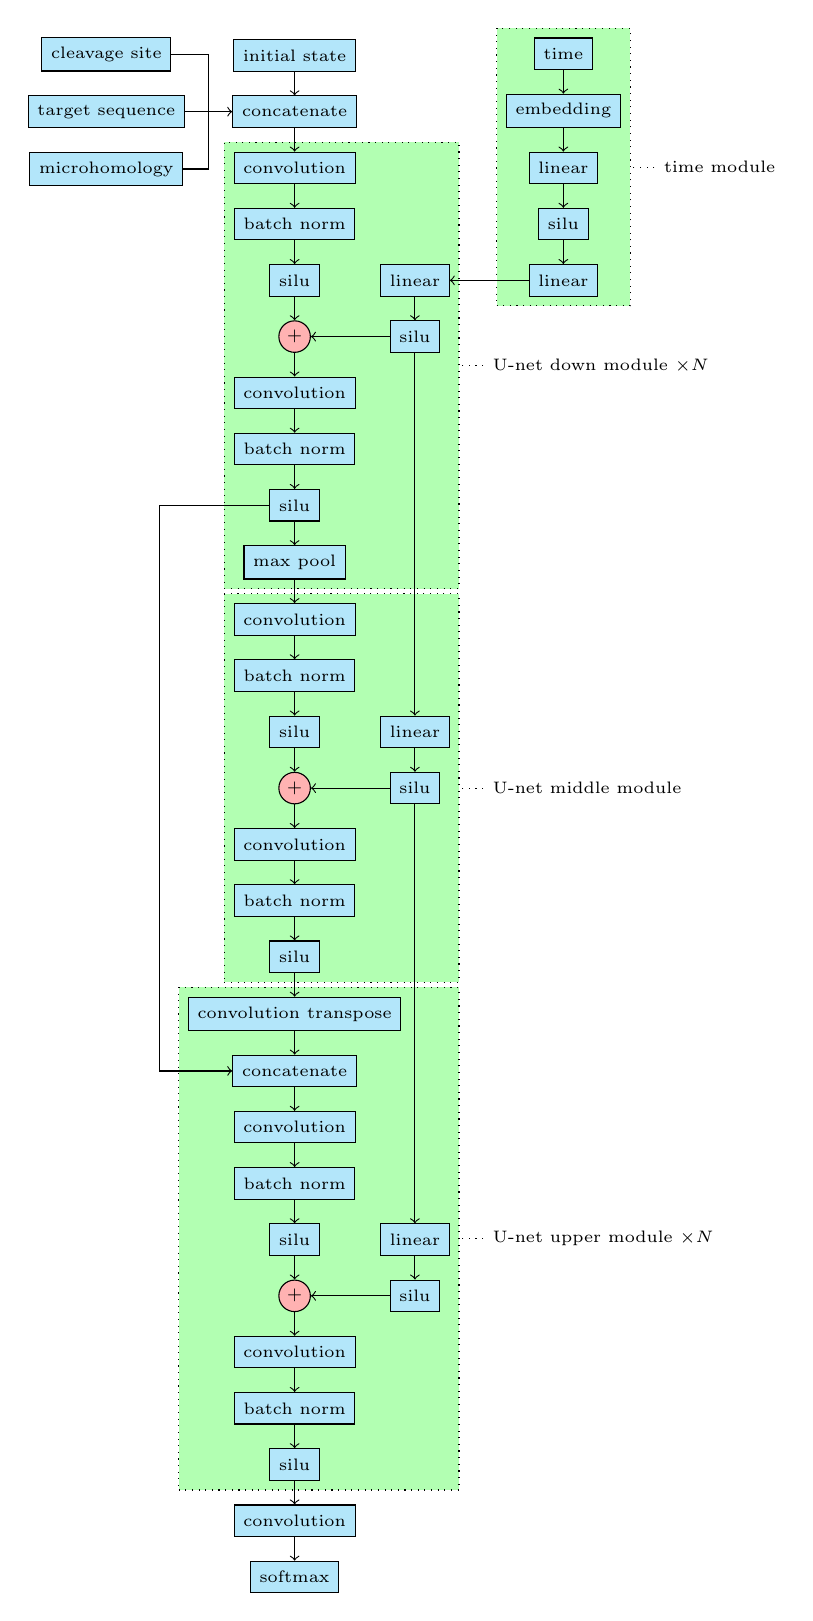
\begin{tikzpicture}
    \node[layer] (initialState) {initial state};
    \node[layer, below=of initialState] (inputConcat) {concatenate};
    \node[layer, below=of inputConcat] (downConv) {convolution};
    \node[layer, below=of downConv] (downNorm) {batch norm};
    \node[layer, below=of downNorm] (downSilu) {silu};
    \node[sum, below=of downSilu] (downSum) {+};
    \node[layer, below=of downSum] (downConv2) {convolution};
    \node[layer, below=of downConv2] (downNorm2) {batch norm};
    \node[layer, below=of downNorm2] (downSilu2) {silu};
    \node[layer, below=of downSilu2] (downMaxPool) {max pool};
    \node[layer, below=of downMaxPool] (middleConv) {convolution};
    \node[layer, below=of middleConv] (middleNorm) {batch norm};
    \node[layer, below=of middleNorm] (middleSilu) {silu};
    \node[sum, below=of middleSilu] (middleSum) {+};
    \node[layer, below=of middleSum] (middleConv2) {convolution};
    \node[layer, below=of middleConv2] (middleNorm2) {batch norm};
    \node[layer, below=of middleNorm2] (middleSilu2) {silu};
    \node[layer, below=of middleSilu2] (upConvTrans) {convolution transpose};
    \node[layer, below=of upConvTrans] (upCat) {concatenate};
    \node[layer, below=of upCat] (upConv) {convolution};
    \node[layer, below=of upConv] (upNorm) {batch norm};
    \node[layer, below=of upNorm] (upSilu) {silu};
    \node[sum, below=of upSilu] (upSum) {+};
    \node[layer, below=of upSum] (upConv2) {convolution};
    \node[layer, below=of upConv2] (upNorm2) {batch norm};
    \node[layer, below=of upNorm2] (upSilu2) {silu};
    \node[layer, below=of upSilu2] (outConv) {convolution};
    \node[layer, below=of outConv] (outSoftmax) {softmax};
    \graph {
      (initialState) -> (inputConcat) -> (downConv) -> (downNorm) -> (downSilu) -> (downSum) -> (downConv2) -> (downNorm2) -> (downSilu2) -> (downMaxPool) -> (middleConv) -> (middleNorm) -> (middleSilu) -> (middleSum) -> (middleConv2) -> (middleNorm2) -> (middleSilu2) -> (upConvTrans) -> (upCat) -> (upConv) -> (upNorm) -> (upSilu) -> (upSum) -> (upConv2) -> (upNorm2) -> (upSilu2) -> (outConv) -> (outSoftmax);
    };

    \coordinate[left=of inputConcat] (conditionAnchor);
    \node[layer, left=of conditionAnchor] (targetSeq) {target sequence};
    \node[layer, above=of targetSeq] (cleavageSite) {cleavage site};
    \node[layer, below=of targetSeq] (microhomology) {microhomology};
    \graph {
      (targetSeq) -- (conditionAnchor) -> (inputConcat);
      (cleavageSite) --[to path={-| (\tikztotarget)}] (conditionAnchor);
      (microhomology) --[to path={-| (\tikztotarget)}] (conditionAnchor);
    };
  
    
    \node[layer, right=10mm of downSum] (downTimeSilu) {silu};
    \node[layer, above=of downTimeSilu] (downTimeLinear) {linear};
    \node[layer] (middleTimeSilu) at (middleSum-|downTimeSilu) {silu};
    \node[layer, above=of middleTimeSilu] (middleTimeLinear) {linear};
    \node[layer] (upTimeSilu) at (upSum-|middleTimeSilu) {silu};
    \node[layer, above=of upTimeSilu] (upTimeLinear) {linear};
    \node[layer, right=10mm of downTimeLinear] (initTimeLinear2) {linear};
    \node[layer, above=of initTimeLinear2] (initTimeSilu) {silu};
    \node[layer, above=of initTimeSilu] (initTimeLinear) {linear};
    \node[layer, above=of initTimeLinear] (initTimeEmb) {embedding};
    \node[layer, above=of initTimeEmb] (time) {time};
    \graph {
      (time) -> (initTimeEmb) -> (initTimeLinear) -> (initTimeSilu) -> (initTimeLinear2) -> (downTimeLinear) -> (downTimeSilu) -> (middleTimeLinear) -> (middleTimeSilu) -> (upTimeLinear) -> (upTimeSilu);
      (downTimeSilu) -> (downSum);
      (middleTimeSilu) -> (middleSum);
      (upTimeSilu) -> (upSum)
    };
    
    \draw[->] (downSilu2) -- ($(downSilu2.west) + (-14mm,0)$) |- (upCat);

    \begin{pgfonlayer}{background}
      \node[bkg, fit=(downConv)(downNorm)(downSilu)(downSum)(downConv2)(downNorm2)(downSilu2)(downMaxPool)(downTimeLinear)(downTimeSilu)] (grpDownMod) {};
      \node[annot, right=of grpDownMod] (grpDownModName) {U-net down module $\times N$};
      \draw[dotted] (grpDownModName) -- (grpDownMod);
    \end{pgfonlayer}

    
    \begin{pgfonlayer}{background}
      \node[bkg, fit=(middleConv)(middleNorm)(middleSilu)(middleSum)(middleConv2)(middleNorm2)(middleSilu2)(middleTimeLinear)(middleTimeSilu)] (grpMiddleMod) {};
      \node[annot, right=of grpMiddleMod] (grpMiddleModName) {U-net middle module};
      \draw[dotted] (grpMiddleModName) -- (grpMiddleMod);
    \end{pgfonlayer}

    
    \begin{pgfonlayer}{background}
      \node[bkg, fit=(upConvTrans)(upCat)(upConv)(upNorm)(upSilu)(upSum)(upConv2)(upNorm2)(upSilu2)(upTimeSilu)(upTimeLinear)] (grpUpMod) {};
      \node[annot, right=of grpUpMod] (grpUpModName) {U-net upper module $\times N$};
      \draw[dotted] (grpUpModName) -- (grpUpMod);
    \end{pgfonlayer}

    \begin{pgfonlayer}{background}
      \node[bkg, fit=(time)(initTimeEmb)(initTimeLinear)(initTimeSilu)(initTimeLinear2)] (grpTimeMod) {};
      \node[annot, right=of grpTimeMod] (grpTimeModName) {time module};
      \draw[dotted] (grpTimeModName) -- (grpTimeMod);
    \end{pgfonlayer}
  \end{tikzpicture}
  \caption{The CRIfuser architecture.}\label{fig:crifuser_architecture} 
\end{figure}

\subsection{Prediction of the editing profile}

CRIfuser as well as other diffusion-based models is a sampler by nature. It predicts editing outcomes one at a time. By repeatedly running CRIfuser, one gets lots of editing outcomes which landscape the whole profile. However, the above method is neither efficient nor accurate. To accurately obtain the editing profile, we first predict the editing profile at each step of the reverse diffusion conditioned on all possible outcomes of the previous step, and then sum out the conditioning on the outcome of the previous step by the marginal profile of the previous step. This gives us an accurate marginal profile of the current step. To speed up the prediction of the editing profile, we apply the optimization of contraction order of tensor products \cite{smith2018opt_einsum}. We also implement an interpolation-based approximation of the editing profile. In detail, we perform a grid-sampling with a given step along each dimension of the diffusion space (the upstream and downstream ligation ends). For our $32\times 32$ diffusion space, a step $n$ will sample $\lfloor32/n\rfloor\times \lfloor32/n\rfloor$ outcomes evenly arranged in the diffusion space. Then CRIfuser predicts the editing profile conditioned on all the sampled outcomes. Before summing out the conditioning on the sampled outcomes, we distribute the weights of the non-sampled outcomes to the sampled ones based on the distance-based linear interpolation. We use this interpolation-based approximation exclusively in the Shapley additive explanations.

\subsection{Continuous-time discrete-space diffusion model}

We first introduce some notations for the discrete-space diffusion model. We denote the path distribution over continuous time interval $[0, T]$ as $q$. Let $q_t$ be the marginal distribution of $q$ at time step $t$. Let $q_{t|s}$ be the conditional distribution of time step $t$ given time step $s$. The projection of $q$ to a single dimension $1\le d\le D$ is denoted by $q^{(d)}$. The original discrete-space diffusion model is based on discrete time step (DTDS) \cite{austin2021structured}. Further work generalize the discrete-space diffusion model to continuous time (CTDS) \cite{campbell2022continuous,zhao2024unified}. We choose to use the CTDS diffusion model for two reasons.
\begin{enumerate}
  \item Generally, $q_0$ cannot be decomposed to the product of the marginal distribution of each dimension. Thus, $q_{0|t}$ used in each iteration of the training process of the DTDS diffusion model cannot be decomposed as well. Directly parameterizing $q_{0|t}$ on all dimensions is not efficient, and even infeasible in the high dimensional case for the DTDS diffusion model. The workaround is to parameterize $q_{0|t}\qty(x_0|x_t)$ as the product of marginal distributions $\prod_{d=1}^D p^{\theta,(d)}_{0|t}\qty(x_0^{(d)}\middle|x_t)$, which neglects the dependencies between dimensions. The CTDS diffusion model has not this problem and can parameteriz $q_{0|t}$ smoothly.

  \item The DTDS model is trained over specific time steps in a given denoise scheduler. Use a different scheduler from training for inference is possible, but may decrease the accuracy of the model. The CTDS diffusion model is trained over the whole time interval, thereby giving more freedom in the choice of inference denoise scheduler.
\end{enumerate}

Following \cite{zhao2024unified}, we use the setting that the diffusion in dimensions are independent, and the forward diffusion process of the diffusion model is
\begin{eqnarray}\label{eq:InterpolarQ}
  q^{(d)}_{t|s}\qty(x^{(d)}_t\middle|x^{(d)}_s) = \alpha^{(d)}_{t|s} \delta\qty(x^{(d)}_t, x^{(d)}_s) + \qty(1 - \alpha^{(d)}_{t|s})\bar{q}^{(d)}\qty(x^{(d)}_t),
\end{eqnarray}
where $\bar{q}^{(d)}$ is the stable distribution of the forward process, and
\begin{eqnarray*}
\lim_{t-s\to+\infty}\alpha^{(d)}_{t|s} = 0
\end{eqnarray*}
promises that the forward diffusion process becomes completely random for large time. This selection greatly simplify the calculation of $q^{(d)}_{s|0,t}\qty(x^{(d)}_s\middle|x^{(d)}_0,x^{(d)}_t)$\cite{zhao2024unified}.
\begin{eqnarray}\label{eq:sOn0tq}
&&q^{(d)}_{s|0,t}\qty(x^{(d)}_s\middle|x^{(d)}_0, x^{(d)}_t)=\frac{q^{(d)}_{t|s}\qty(x^{(d)}_t\middle|x^{(d)}_s)q^{(d)}_{s|0}\qty(x^{(d)}_s\middle|x^{(d)}_0)}{q^{(d)}_{t|0}\qty(x^{(d)}_t\middle|x^{(d)}_0)}\nonumber\\
&&=\begin{cases}
    \qty(1-\lambda^{(d)}_{t|s})\delta\qty(\mathbf{x}^{(d)}_s, \mathbf{x}^{(d)}_t) + \lambda^{(d)}_{t|s}\bar{q}^{(d)}\qty(x^{(d)}_s), & x_0^{(d)}=x^{(d)}_t,\\
    \begin{aligned}
      &\qty(1-\mu^{(d)}_{t|s})\delta\qty(\mathbf{x}^{(d)}_s, \mathbf{x}^{(d)}_0) + \mu^{(d)}_{t|s}\alpha^{(d)}_{t|s}\delta\qty(\mathbf{x}^{(d)}_s, \mathbf{x}^{(d)}_t) \\
      &+ \mu^{(d)}_{t|s}\qty(1-\alpha^{(d)}_{t|s})\bar{q}^{(d)}\qty(x^{(d)}_s),
    \end{aligned}
    & x_0^{(d)}\neq x_t^{(d)},
\end{cases}
\end{eqnarray}
where
\begin{eqnarray*}
    &&\lambda^{(d)}_{t|s}\coloneq\frac{\qty(1-\alpha^{(d)}_{s|0})\qty(1-\alpha^{(d)}_{t|s})\bar{q}^{(d)}\qty(x^{(d)}_t)}{\alpha^{(d)}_{t|0} + \qty(1-\alpha^{(d)}_{t|0})\bar{q}^{(d)}\qty(x^{(d)}_t)},\\
    &&\mu^{(d)}_{t|s}=\frac{1-\alpha^{(d)}_{s|0}}{1-\alpha^{(d)}_{t|0}}.
\end{eqnarray*}

The authors in \cite{campbell2022continuous} suggest the Markov forward process ($q^{(d)}_t$ is a row vector)
\begin{eqnarray*}
\frac{d q^{(d)}_t}{dt}=q^{(d)}_t R^{(d)}_t,  
\end{eqnarray*}
where $R^{(d)}_t$ is the transition rate at time $t$. If $R^{(d)}_t$ commutes for all time $t$, then the solution is ($s$ for rows and $t$ for columns)
\begin{eqnarray*}
q^{(d)}_{t|s} = e^{\int_s^t R^{(d)}_\tau d\tau}.  
\end{eqnarray*}
To achieve the commutation condition, they further suggest the forward transition rate $R^{(d)}_t$ of the form (for simplicity, we assume the time-based scale $\beta_t$ is independent of dimension $d$)
\begin{eqnarray*}
R^{(d)}_t\coloneqq \beta_t \bar{R}^{(d)},  
\end{eqnarray*}
where $\bar{R}^{(d)}$ is a constant transition rate, and $\beta_t$ is a time-dependent scalar. If further require $\qty(\bar{R}^{(d)})^2 = \bar{R}^{(d)}$, then
\begin{eqnarray*}
  q^{(d)}_{t|s} = e^{\bar{R}^{(d)}\int_s^t \beta_\tau d\tau} = I + (1 - e^{-\int_s^t \beta_\tau d\tau})\bar{R}^{(d)}.
\end{eqnarray*}
Thus, Eq. \eqref{eq:InterpolarQ} is actually
\begin{eqnarray}\label{eq:RtExpress}
\bar{R}^{(d)} = \mathbf{1}\bar{q}^{(d)} - I,  
\end{eqnarray}
where $\mathbf{1}$ is a column vector of the size of the total discrete space whose components are all one. To see this, note that
\begin{eqnarray*}
    \qty(I - \mathbf{1}\bar{q}^{(d)})^2 = I - 2 * \mathbf{1}\bar{q}^{(d)} + \mathbf{1}\bar{q}^{(d)}\mathbf{1}\bar{q}^{(d)} = I - \mathbf{1}\bar{q}^{(d)}.
\end{eqnarray*}
Therefore,
\begin{eqnarray}\label{eq:ForDiff}
    &&q^{(d)}_{t|s} = e^{\bar{R}^{(d)}\int_s^t \beta_\tau d\tau} = I + \qty(1 - e^{-\int_s^t \beta_\tau d\tau})\bar{R}^{(d)} \nonumber\\
    && = I + \qty(1 - e^{-\int_s^t \beta_\tau d\tau})\qty(\mathbf{1}\bar{q}^{(d)} - I) \nonumber\\
    && = e^{-\int_s^t \beta_\tau d\tau} I + \qty(1 - e^{-\int_s^t \beta_\tau d\tau})\mathbf{1}\bar{q}^{(d)},
\end{eqnarray}
which is Eq. \eqref{eq:InterpolarQ} with $\alpha^{(d)}_{t|s} = e^{-\int_s^t \beta_\tau d\tau}$.

According to \cite{zhao2024unified}, the transition rate of the reverse diffusion process $\widehat{R}_t$ is calculated by
\begin{eqnarray}\label{EqDivParaHatR}
    &&\widehat{R}_t\qty(y_t\middle|x_t)=\sum_{d=1}^D R^{(d)}_t\qty(x^{(d)}_t\middle| y^{(d)}_t)\delta\qty(x^{(\setminus d)}_t,y^{(\setminus d)}_t) g^{(d)}_t\qty(y^{(d)}_t\middle|x_t)\nonumber\\
    &&=\sum_{d=1}^D \frac{R^{(d)}_t\qty(x^{(d)}_t\middle| y^{(d)}_t)\delta\qty(x^{(\setminus d)}_t,y^{(\setminus d)}_t)}{g^{(d)}_t\qty(x^{(d)}_t\middle|y_t)},\\
    &&g^{(d)}_t\qty(y^{(d)}_t\middle|x_t)\coloneq \frac{q_t\qty(y^{(d)}_t, x^{(\setminus d)}_t)}{q_t\qty(x_t)} = \sum_{x^{(d)}_0}\frac{q^{(d)}_{t|0}\qty(y^{(d)}_t\middle|x^{(d)}_0)}{q^{(d)}_{t|0}\qty(x^{(d)}_t\middle|x^{(d)}_0)}q^{(d)}_{0|t}\qty(x^{(d)}_0\middle| x_t),
\end{eqnarray}
where $x^{(\setminus d)}_t$ means all dimensions except $d$.

The authors in \cite{zhao2024unified} suggest to use the negative ELBO as part of the loss function. They parameterize the negative ELBO as ($\Delta t\equiv T / K$ and $t_k\equiv k\Delta t$)
\begin{eqnarray*}
  &&\mathcal{L}^\text{CT}(\theta)\coloneq \lim_{K\to+\infty}\sum_{k=0}^{K-1} - \mathbb{E}_{q_{t_{k+1}}\qty(x_{t_{k+1}})}\mathbb{E}_{q_{t_k|t_{k+1}}\qty(x_{t_k}|x_{t_{k+1}})}\nonumber\\
  &&\log \qty(\delta\qty(x_{t_k},x_{t_{k+1}}) + \widehat{R}_{t_{k+1}}^\theta\qty(x_{t_k}|x_{t_{k+1}})\Delta t + o(\Delta t))\\
  &&= T\mathbb{E}_{\mathcal{U}(t;0,T)}\mathbb{E}_{q_t\qty(x_t)}\qty[\sum_{y_t\neq x_t}\widehat{R}_t^\theta\qty(y_t\middle|x_t) - \sum_{y_t\neq x_t}R_t\qty(y_t\middle|x_t)\log\widehat{R}_t^\theta\qty(x_t\middle|y_t)] + C,
\end{eqnarray*}
where
\begin{eqnarray}
  &&\widehat{R}^\theta_t\qty(y_t\middle|x_t)\coloneqq\sum_{d=1}^D R^{(d)}_t\qty(x^{(d)}_t\middle| y^{(d)}_t)\delta\qty(x^{(\setminus d)}_t,y^{(\setminus d)}_t) g^{\theta,(d)}_t\qty(y^{(d)}_t\middle|x_t),\label{eq:RthetaSingle}\\
  &&g^{\theta,(d)}_t\qty(y^{(d)}_t\middle|x_t)\coloneq\sum_{x^{(d)}_0}\frac{q^{(d)}_{t|0}\qty(y^{(d)}_t\middle|x^{(d)}_0)}{q^{(d)}_{t|0}\qty(x^{(d)}_t\middle|x^{(d)}_0)}p^{\theta,(d)}_{0|t}\qty(x^{(d)}_0\middle| x_t).
\end{eqnarray}
Let
\begin{eqnarray*}
  &&\mathcal{L}_1^\text{CT}(\theta) \coloneqq T\mathbb{E}_{\mathcal{U}(t;0,T)}\mathbb{E}_{q_t\qty(x_t)}\sum_{y_t\neq x_t}\widehat{R}^\theta_t\qty(y_t\middle|x_t),\\
  &&\mathcal{L}_2^\text{CT}(\theta) \coloneqq -T\mathbb{E}_{\mathcal{U}(t;0,T)}\mathbb{E}_{q_t\qty(x_t)} \sum_{y_t\neq x_t}R_t\qty(y_t\middle|x_t)\log\widehat{R}_t^\theta\qty(x_t\middle|y_t).
\end{eqnarray*}
Then
\begin{eqnarray*}
  \mathcal{L}^\text{CT}(\theta) = \mathcal{L}_1^\text{CT}(\theta) + \mathcal{L}_2^\text{CT}(\theta) + C.
\end{eqnarray*}
By \cite{zhao2024unified}, $\mathcal{L}_1^\text{CT}(\theta)$ can be efficiently calculated by
\begin{eqnarray}\label{eq:LossFirstTerm}
  \sum_{y_t\neq x_t}\widehat{R}_t^\theta\qty(y_t|x_t)=\beta_t\sum_{d=1}^D\bar{q}^{(d)}\qty(x^{(d)}_t)\sum_{y^{(d)}_t}g^{\theta,(d)}_t\qty(y^{(d)}_t\middle|x_t) + C.
\end{eqnarray}

\subsection{The double-sampling loss function}

In each training iteration of the diffusion model, $x_t$ is fixed through sampling $x_0$, $t$ and $x_t$ sequentially. However, $y_t$ can be any value not equaling $x_t$. The calculation of $\widehat{R}^\theta_t\qty(x_t\middle|y_t)$ for each $y_t\neq x_t$ needs an expensive network inference to get $p^{\theta,(d)}_{0|t}\qty(\cdot\middle|y_t)$. The authors of \cite{campbell2022continuous} solve this problem by sampling $y_t$ given $x_t$ according to
\begin{eqnarray}
  S_t\qty(y_t|x_t) \coloneqq \frac{R_t\qty(y_t|x_t)}{-R_t\qty(x_t|x_t)}.
\end{eqnarray}
We call this the double-sampling loss function.
\begin{eqnarray*}
  \dot{\mathcal{L}}_2^\text{CT}(\theta) \coloneqq T\mathbb{E}_{\mathcal{U}(t;0,T)}\mathbb{E}_{q_t\qty(x_t)}\mathbb{E}_{S_t\qty(y_t\middle|x_t)}R_t\qty(x_t|x_t)\log\widehat{R}_t^\theta\qty(x_t\middle|y_t).
\end{eqnarray*}
Note that the double-sampling loss function still needs two forward passes to calculate $\widehat{R}_t^\theta\qty(\cdot\middle|x_t)$ for $\mathcal{L}_1^\text{CT}(\theta)$ and $\widehat{R}_t^\theta\qty(\cdot\middle|y_t)$ for $\dot{\mathcal{L}}_2^\text{CT}(\theta)$. To achieve only one forward pass, the authors of \cite{campbell2022continuous} approximate $q_t(x_t)$ by $\sum_{x_t}q_t(x_t)S_t\qty(y_t|x_t)$. Then
\begin{eqnarray*}
  &&\mathcal{L}_1^\text{CT}(\theta)\approx \dot{\mathcal{L}}_1^\text{CT}(\theta) \coloneqq T\mathbb{E}_{\mathcal{U}(t;0,T)}\mathbb{E}_{q_t\qty(x_t)}\mathbb{E}_{S_t\qty(y_t\middle|x_t)}\sum_{z_t\neq y_t}\widehat{R}_t^\theta\qty(z_t\middle|y_t).
\end{eqnarray*}
Together with Eqs. \eqref{eq:RtExpress}, \eqref{eq:RthetaSingle}, \eqref{eq:LossFirstTerm},
\begin{eqnarray}\label{eq:ELBOoriginal}
&&\dot{\mathcal{L}}_1^\text{CT}(\theta) = T\mathbb{E}_{\mathcal{U}(t;0,T)}\beta_t\mathbb{E}_{q_t\qty(x_t)}\mathbb{E}_{S_t\qty(y_t\middle|x_t)}\sum_{d=1}^D\bar{q}^{(d)}\qty(y^{(d)}_t)\sum_{z^{(d)}_t}g^{\theta,(d)}_t\qty(z^{(d)}_t\middle|y_t),\\
&&\dot{\mathcal{L}}_2^\text{CT}(\theta) = -T\mathbb{E}_{\mathcal{U}(t;0,T)}\beta_t\mathbb{E}_{q_t\qty(x_t)}\mathbb{E}_{S_t\qty(y_t\middle|x_t)}\qty(\sum_{d=1}^D\sum_{z^{(d)}_t\neq x^{(d)}_t}\bar{q}^{(d)}\qty(z^{(d)}_t))\nonumber\\
&&\log\qty(\sum_{d=1}^D \bar{q}^{(d)}\qty(y^{(d)}_t)\delta\qty(y^{(\setminus d)}_t,x^{(\setminus d)}_t) g^{\theta,(d)}_t\qty(x^{(d)}_t\middle|y_t)) + C.
\end{eqnarray}

\subsection{The importance-sampling loss function}
The authors of \cite{zhao2024unified} use the importance sampling to handle the second term of $\mathcal{L}^\text{CT}(\theta)$. The original derivation is quite complex. We give a simplified version.
\begin{eqnarray*}
  &&T\mathbb{E}_{\mathcal{U}(t;0,T)}\mathbb{E}_{q_t\qty(x_t)}\sum_{y_t\neq x_t}R_t\qty(y_t\middle|x_t)\log\widehat{R}_t^\theta\qty(x_t|y_t)\\
  &&=T\mathbb{E}_{\mathcal{U}(t;0,T)}\mathbb{E}_{q_0\qty(x_0)}\mathbb{E}_{q_{t|0}\qty(x_t|x_0)}\mathbb{E}_{q_{t|0}\qty(y_t|x_0)}\\
  &&\qty[1-\delta\qty(x_t, y_t)]\frac{1}{q_{t|0}\qty(y_t|x_0)}R_t\qty(y_t\middle|x_t)\log\widehat{R}_t^\theta\qty(x_t|y_t)\\
  &&=T\mathbb{E}_{\mathcal{U}(t;0,T)}\mathbb{E}_{q_0\qty(x_0)}\mathbb{E}_{q_{t|0}\qty(y_t|x_0)}\sum_{x_t\neq y_t}\frac{q_{t|0}\qty(x_t|x_0)}{q_{t|0}\qty(y_t|x_0)}R_t\qty(y_t\middle|x_t)\log\widehat{R}_t^\theta\qty(x_t|y_t)\\
  &&=T\mathbb{E}_{\mathcal{U}(t;0,T)}\mathbb{E}_{q_0\qty(x_0)}\mathbb{E}_{q_{t|0}\qty(y_t|x_0)}\\
  &&\sum_{d=1}^D\sum_{x^{(d)}_t\neq y^{(d)}_t}\frac{q^{(d)}_{t|0}\qty(x^{(d)}_t\middle|x^{(d)}_0)}{q^{(d)}_{t|0}\qty(y^{(d)}_t|x^{(d)}_0)}R^{(d)}_t\qty(y^{(d)}_t\middle|x^{(d)}_t)\log R^{(d)}_t\qty(y^{(d)}_t\middle|x^{(d)}_t)g^{\theta,(d)}_t\qty(x^{(d)}_t\middle|y_t)\\
  &&=T\mathbb{E}_{\mathcal{U}(t;0,T)}\beta_t\mathbb{E}_{q_0\qty(x_0)}\mathbb{E}_{q_{t|0}\qty(y_t|x_0)}\\
  &&\sum_{d=1}^D\bar{q}^{(d)}\qty(y^{(d)}_t)\sum_{x^{(d)}_t\neq y^{(d)}_t}\frac{q^{(d)}_{t|0}\qty(x^{(d)}_t\middle|x^{(d)}_0)}{q^{(d)}_{t|0}\qty(y^{(d)}_t|x^{(d)}_0)}\log g^{\theta,(d)}_t\qty(x^{(d)}_t\middle|y_t) + C.
\end{eqnarray*}
Exchange $x_t$ and $y_t$ in the last equality, and use the fact that
\begin{eqnarray}\label{eq:GthetaVanish}
  &&\log g^{\theta,(d)}_t\qty(x^{(d)}_t\middle|x_t)=\log \sum_{x^{(d)}_0}\frac{q^{(d)}_{t|0}\qty(x^{(d)}_t\middle|x^{(d)}_0)}{q^{(d)}_{t|0}\qty(x^{(d)}_t\middle|x^{(d)}_0)}p^{\theta,(d)}_{0|t}\qty(x^{(d)}_0\middle| x_t)\nonumber\\
  &&\equiv \log \sum_{x^{(d)}_0}p^{\theta,(d)}_{0|t}\qty(x^{(d)}_0\middle| x_t) \equiv \log 1 \equiv 0,
\end{eqnarray}
we have the importance-sampling loss function as
\begin{eqnarray}\label{eq:ELBOunified}
  &&\bar{\mathcal{L}}_2^\text{CT}(\theta)\coloneqq -T\mathbb{E}_{\mathcal{U}(t;0,T)}\beta_t\mathbb{E}_{q_{0,t}\qty(x_0,x_t)}\nonumber\\
  &&\sum_{d=1}^D\bar{q}^{(d)}\qty(x^{(d)}_t)\sum_{y^{(d)}_t}\frac{q^{(d)}_{t|0}\qty(y^{(d)}_t\middle|x^{(d)}_0)}{q^{(d)}_{t|0}\qty(x^{(d)}_t\middle|x^{(d)}_0)}\log g^{\theta,(d)}_t\qty(y^{(d)}_t\middle|x_t) + C.
\end{eqnarray}

\subsection{Our forward loss function}
We propose a simpler method as follows. By Eq. \eqref{EqDivParaHatR}, define the new parameterization of the reverse transition rate as
\begin{eqnarray}
  \tilde{R}^\theta_t\qty(x_t\middle|y_t)\coloneq\sum_{d=1}^D \frac{R^{(d)}_t\qty(y^{(d)}_t\middle| x^{(d)}_t)\delta\qty(x^{(\setminus d)}_t ,y^{(\setminus d)}_t)}{g^{\theta,(d)}_t\qty(y^{(d)}_t\middle|x_t)}.
\end{eqnarray}
Replace $\widehat{R}^\theta_t\qty(x_t\middle|y_t)$ by $\tilde{R}^\theta_t\qty(x_t\middle|y_t)$ in $\mathcal{L}_2^\text{CT}(\theta)$.
\begin{eqnarray}\label{EqBetterNgELBO}
  \widetilde{\mathcal{L}}_2^\text{CT}(\theta)\coloneq -T\mathbb{E}_{\mathcal{U}(t;0,T)}\mathbb{E}_{q_t\qty(x_t)}\sum_{y_t\neq x_t}R_t\qty(y_t\middle|x_t)\log\tilde{R}_t^\theta\qty(x_t\middle|y_t) + C.
\end{eqnarray}
Then all one needs is to calculate $g^\theta_t(y_t|x_t)$, which only needs a single pass for $p^\theta_{0|t}(\cdot|x_t)$. We call this the forward loss function.

We find that the second term upon the forward diffusion in Eq. \eqref{eq:ForDiff} can be efficiently calculated.
\begin{eqnarray*}
  &&- \sum_{y_t\neq x_t}R_t\qty(y_t\middle|x_t)\log\tilde{R}_t^\theta\qty(x_t\middle|y_t)\\
  &&=-\sum_{d=1}^D\sum_{y^{(d)}_t\neq x^{(d)}_t}R^{(d)}_t\qty(y^{(d)}_t\middle|x^{(d)}_t)\log\frac{R_t^{(d)}\qty(y^{(d)}_t\middle|x^{(d)}_t)}{g^{\theta,(d)}_t\qty(y^{(d)}_t\middle|x_t)}\\
  &&=\sum_{d=1}^D\sum_{y^{(d)}_t\neq x^{(d)}_t}R^{(d)}_t\qty(y^{(d)}_t\middle|x^{(d)}_t)\log g^{\theta,(d)}_t\qty(y^{(d)}_t\middle|x_t) + C\\
  &&=\beta_t\sum_{d=1}^D\sum_{y^{(d)}_t}\bar{q}^{(b)}\qty(y^{(d)}_t) g^{\theta,(d)}_t\qty(y^{(d)}_t\middle|x_t) + C.
\end{eqnarray*}
Thus, together with \eqref{eq:GthetaVanish}, we have
\begin{eqnarray}\label{eq:ELBOforward}
  \widetilde{\mathcal{L}}_2^\text{CT}(\theta)=T\mathbb{E}_{\mathcal{U}(t;0,T)}\beta_t\mathbb{E}_{q_t\qty(x_t)}\sum_{d=1}^D\sum_{y^{(d)}_t}\bar{q}^{(b)}\qty(y^{(d)}_t) g^{\theta,(d)}_t\qty(y^{(d)}_t\middle|x_t) + C.
\end{eqnarray}



\subsection{Our reverse loss function}

By \cite{campbell2022continuous} ($\Delta t\equiv T / K$ and $t_k\equiv k\Delta t$),
\begin{eqnarray*}
  \mathcal{L}^{DT}(\theta) = - \sum_{k=0}^{K - 1} \mathbb{E}_{q_{t_k,t_{k+1}}\qty(x_{t_k},x_{t_{k+1}})}\log p^\theta_{t_k|t_{k+1}}\qty(x_{t_k}|x_{t_{k+1}}).
\end{eqnarray*}
The authors of \cite{campbell2022continuous} sample $x_{t_k}$, and expand the expectation over $x_{t_{k+1}}$.
\begin{eqnarray*}
&&\mathbb{E}_{q_{t_k,t_{k+1}}\qty(x_{t_k},x_{t_{k+1}})}\log p^\theta_{t_k|t_{k+1}}\qty(x_{t_k}|x_{t_{k+1}}) \\
&&=\mathbb{E}_{q_{t_k}\qty(x_{t_k})}\mathbb{E}_{q_{t_{k+1}|t_k}\qty(x_{t_{k+1}}|x_{t_k})}\\
&&\log \qty(\delta\qty(x_{t_k},x_{t_{k+1}}) + \widehat{R}_{t_{k+1}}^\theta\qty(x_{t_k}|x_{t_{k+1}})\Delta t + o(\Delta t)) \\
&&= \mathbb{E}_{q_{t_k}\qty(x_{t_k})}\sum_{x_{t_{k+1}}}q_{t_{k+1}|t_k}\qty(x_{t_{k+1}}|x_{t_k})\\
&&\log \qty(\delta\qty(x_{t_k},x_{t_{k+1}}) + \widehat{R}_{t_{k+1}}^\theta\qty(x_{t_k}|x_{t_{k+1}})\Delta t + o(\Delta t)) \\
&&= \mathbb{E}_{q_{t_k}\qty(x_{t_k})}\sum_{x_{t_{k+1}}}\qty(\delta\qty(x_{t_k},x_{t_{k+1}}) + R_{t_k}\qty(x_{t_{k+1}}|x_{t_k})\Delta t + o(\Delta t)) \\
&&\log \qty(\delta\qty(x_{t_k},x_{t_{k+1}}) + \widehat{R}_{t_{k+1}}^\theta\qty(x_{t_k}|x_{t_{k+1}})\Delta t + o(\Delta t)) \\
&&= \mathbb{E}_{q_{t_k}\qty(x_{t_k})}\Bigg(\widehat{R}_{t_{k+1}}^\theta\qty(x_{t_k}|x_{t_k})\Delta t \\
&&+ \sum_{x_{t_{k+1}}\neq x_{t_k}}R_{t_k}\qty(x_{t_{k+1}}|x_{t_k})\Delta t \log \qty(\widehat{R}_{t_{k+1}}^\theta\qty(x_{t_k}|x_{t_{k+1}})\Delta t + o(\Delta t)) + o(\Delta t)\Bigg) \\
&&= \mathbb{E}_{q_{t_k}\qty(x_{t_k})}\Bigg(\widehat{R}_{t_{k+1}}^\theta\qty(x_{t_k}|x_{t_k})\Delta t \\
&&+ \sum_{x_{t_{k+1}}\neq x_{t_k}}R_{t_k}\qty(x_{t_{k+1}}|x_{t_k})\Delta t \qty(\log\Delta t + \log \widehat{R}_{t_{k+1}}^\theta\qty(x_{t_k}|x_{t_{k+1}}) + \log(1 + o(1))) \\
&&+ o(\Delta t)\Bigg) \\
&&= \Delta t\mathbb{E}_{q_{t_k}\qty(x_{t_k})}\qty(\widehat{R}_{t_{k+1}}^\theta\qty(x_{t_k}|x_{t_k}) + \sum_{x_{t_{k+1}}\neq x_{t_k}}R_{t_k}\qty(x_{t_{k+1}}|x_{t_k}) \log \widehat{R}_{t_{k+1}}^\theta\qty(x_{t_k}|x_{t_{k+1}})) \\
&&+ o(\Delta t) + C.
\end{eqnarray*}
Thus,
\begin{eqnarray*}
  &&\mathcal{L}^\text{CT}(\theta) = \lim_{\Delta t\to 0}\mathcal{L}^\text{DT}(\theta) \\
  &&= - \lim_{\Delta t\to 0}\sum_{k=0}^{K-1}\Bigg[\Delta t\mathbb{E}_{q_{t_k}\qty(x_{t_k})}\qty(\widehat{R}_{t_{k+1}}^\theta\qty(x_{t_k}|x_{t_k}) + \sum_{x_{t_{k+1}}\neq x_{t_k}}R_{t_k}\qty(x_{t_{k+1}}|x_{t_k}) \log \widehat{R}_{t_{k+1}}^\theta\qty(x_{t_k}|x_{t_{k+1}})) \\
  &&+ o(\Delta t) + C\Bigg]\\
  &&= - \int_0^T \mathbb{E}_{q_t\qty(x_t)}\qty(\widehat{R}_t^\theta\qty(x_t|x_t) + \sum_{y_t\neq x_t}R_t(y_t|x_t)\log\widehat{R}_t^\theta(x_t|y_t))dt + C\\
  &&=\int_0^T \mathbb{E}_{q_t\qty(x_t)}\qty(\sum_{y_t\neq x_t}\widehat{R}_t^\theta\qty(y_t|x_t) - \sum_{y_t\neq x_t}R_t\qty(y_t|x_t)\log\widehat{R}_t^\theta\qty(x_t|y_t))dt + C\\
  &&=T\mathbb{E}_{\mathcal{U}(t;0,T)}\mathbb{E}_{q_t\qty(x_t)}\qty(\sum_{y_t\neq x_t}\widehat{R}_t^\theta\qty(y_t|x_t) - \sum_{y_t\neq x_t}R_t\qty(y_t|x_t)\log\widehat{R}_t^\theta\qty(x_t|y_t)) + C.
\end{eqnarray*}

On the contrary, we choose to sample $x_{t_{k+1}}$, and expand the expectation over $x_{t_k}$.
\begin{eqnarray*}
  &&\mathbb{E}_{q_{t_k,t_{k+1}}\qty(x_{t_k},x_{t_{k+1}})}\log p^\theta_{t_k|t_{k+1}}\qty(x_{t_k}|x_{t_{k+1}}) \\
  &&= \mathbb{E}_{q_{t_{k+1}}\qty(x_{t_{k+1}})}\mathbb{E}_{q_{t_k|t_{k+1}}\qty(x_{t_k}|x_{t_{k+1}})}\\
  &&\log \qty(\delta\qty(x_{t_k},x_{t_{k+1}}) + \widehat{R}_{t_{k+1}}^\theta\qty(x_{t_k}|x_{t_{k+1}})\Delta t + o(\Delta t)) \\
  &&= \mathbb{E}_{q_{t_{k+1}}\qty(x_{t_{k+1}})}\sum_{x_{t_k}}q_{t_k|t_{k+1}}\qty(x_{t_k}|x_{t_{k+1}})\\
  &&\log \qty(\delta\qty(x_{t_k},x_{t_{k+1}}) + \widehat{R}_{t_{k+1}}^\theta\qty(x_{t_k}|x_{t_{k+1}})\Delta t + o(\Delta t)) \\
  &&= \mathbb{E}_{q_{t_{k+1}}\qty(x_{t_{k+1}})}\sum_{x_{t_k}}\qty(\delta\qty(x_{t_k},x_{t_{k+1}}) + \widehat{R}_{t_{k+1}}\qty(x_{t_k}|x_{t_{k+1}})\Delta t + o(\Delta t))\\
  &&\log \qty(\delta\qty(x_{t_k},x_{t_{k+1}}) + \widehat{R}_{t_{k+1}}^\theta\qty(x_{t_k}|x_{t_{k+1}})\Delta t + o(\Delta t)) \\
  &&= \mathbb{E}_{q_{t_{k+1}}\qty(x_{t_{k+1}})}\Bigg(\widehat{R}_{t_{k+1}}^\theta\qty(x_{t_{k+1}}|x_{t_{k+1}})\Delta t \\
  &&+ \sum_{x_{t_k}\neq x_{t_{k+1}}}\widehat{R}_{t_{k+1}}\qty(x_{t_k}|x_{t_{k+1}})\Delta t \log \qty(\widehat{R}_{t_{k+1}}^\theta\qty(x_{t_k}|x_{t_{k+1}})\Delta t + o(\Delta t)) + o(\Delta t)\Bigg) \\
  &&= \mathbb{E}_{q_{t_{k+1}}\qty(x_{t_{k+1}})}\Bigg(\widehat{R}_{t_{k+1}}^\theta\qty(x_{t_{k+1}}|x_{t_{k+1}})\Delta t \\
  &&+ \sum_{x_{t_k}\neq x_{t_{k+1}}}\widehat{R}_{t_{k+1}}\qty(x_{t_k}|x_{t_{k+1}})\Delta t \qty(\log\Delta t + \log \widehat{R}_{t_{k+1}}^\theta\qty(x_{t_k}|x_{t_{k+1}}) + \log(1 + o(1))) + o(\Delta t)\Bigg) \\
  &&= \Delta t\mathbb{E}_{q_{t_{k+1}}\qty(x_{t_{k+1}})}\qty(\widehat{R}_{t_{k+1}}^\theta\qty(x_{t_{k+1}}|x_{t_{k+1}}) + \sum_{x_{t_k}\neq x_{t_{k+1}}}\widehat{R}_{t_{k+1}}\qty(x_{t_k}|x_{t_{k+1}}) \log \widehat{R}_{t_{k+1}}^\theta\qty(x_{t_k}|x_{t_{k+1}})) \\
  &&+ o(\Delta t) + C.
\end{eqnarray*}
Thus,
\begin{eqnarray*}
  &&\widehat{\mathcal{L}}^\text{CT}(\theta) = \lim_{\Delta t\to 0}\mathcal{L}^\text{DT}(\theta) \\
  &&= - \lim_{\Delta t\to 0}\sum_{k=0}^{K-1}\Bigg[\Delta t\mathbb{E}_{q_{t_{k+1}}\qty(x_{t_{k+1}})}\Bigg(\widehat{R}_{t_{k+1}}^\theta\qty(x_{t_{k+1}}|x_{t_{k+1}}) \\
  &&+ \sum_{x_{t_k}\neq x_{t_{k+1}}}\widehat{R}_{t_{k+1}}\qty(x_{t_k}|x_{t_{k+1}}) \log \widehat{R}_{t_{k+1}}^\theta\qty(x_{t_k}|x_{t_{k+1}})\Bigg) + o(\Delta t) + C\Bigg] \\
  &&= - \int_0^T \mathbb{E}_{q_t\qty(x_t)}\qty(\widehat{R}_t^\theta\qty(x_t|x_t) + \sum_{y_t\neq x_t}\widehat{R}_t\qty(y_t|x_t)\log\widehat{R}_t^\theta\qty(y_t|x_t))dt + C\\
  &&=\int_0^T \mathbb{E}_{q_t\qty(x_t)}\qty(\sum_{y_t\neq x_t}\widehat{R}_t^\theta\qty(y_t|x_t) - \sum_{y_t\neq x_t}\widehat{R}_t\qty(y_t|x_t)\log\widehat{R}_t^\theta\qty(y_t|x_t))dt + C\\
  &&=T\mathbb{E}_{\mathcal{U}(t;0,T)}\mathbb{E}_{q_t\qty(x_t)}\qty(\sum_{y_t\neq x_t}\widehat{R}_t^\theta\qty(y_t|x_t) - \sum_{y_t\neq x_t}\widehat{R}_t\qty(y_t|x_t)\log\widehat{R}_t^\theta\qty(y_t|x_t)) + C\\
  &&=\mathcal{L}_1^\text{CT}(\theta) - T\mathbb{E}_{\mathcal{U}(t;0,T)}\mathbb{E}_{q_t\qty(x_t)}\sum_{y_t\neq x_t}\widehat{R}_t\qty(y_t|x_t)\log\widehat{R}_t^\theta\qty(y_t|x_t) + C\\
  &&\eqqcolon \mathcal{L}_1^\text{CT}(\theta) + \widehat{\mathcal{L}}_2^\text{CT}(\theta).
\end{eqnarray*}
We call this the reverse loss function. We find that the second term of the reverse loss function can be efficiently calculated as
\begin{eqnarray*}
  && - \sum_{y_t\neq x_t}\widehat{R}_t\qty(y_t\middle|x_t)\log\widehat{R}_t^\theta\qty(y_t\middle|x_t) \\
  && = - \sum_{d=1}^D\sum_{y^{(d)}_t\neq x^{(d)}_t}R_t\qty(x^{(d)}_t\middle|y^{(d)}_t)g_t^{(d)}\qty(y^{(d)}_t\middle|x_t)\log\qty[R_t\qty(x^{(d)}_t\middle|y^{(d)}_t)g_t^{\theta, (d)}\qty(y^{(d)}_t\middle|x_t)] \\
  && = - \sum_{d=1}^D\sum_{y^{(d)}_t\neq x^{(d)}_t}R_t\qty(x^{(d)}_t\middle|y^{(d)}_t)g_t^{(d)}\qty(y^{(d)}_t\middle|x_t)\log g_t^{\theta, (d)}\qty(y^{(d)}_t\middle|x_t) + C \\
  && = - \beta_t\sum_{d=1}^D \bar{q}^{(d)}\qty(x^{(d)}_t)\sum_{y^{(d)}_t}g_t^{(d)}\qty(y^{(d)}_t\middle|x_t)\log g_t^{\theta, (d)}\qty(y^{(d)}_t\middle|x_t) + C.
\end{eqnarray*}
Thus,
\begin{eqnarray}\label{eq:ELBOreverse}
  &&\widehat{\mathcal{L}}_2^\text{CT}(\theta) =\nonumber\\
  &&-T\mathbb{E}_{\mathcal{U}(t;0,T)}\beta_t\mathbb{E}_{q_t\qty(x_t)}\sum_{d=1}^D\bar{q}^{(d)}\qty(x^{(d)}_t)\sum_{y^{(d)}_t}\qty[g_t^{(d)}\qty(y^{(d)}_t\middle|x_t)\log g_t^{\theta, (d)}\qty(y^{(d)}_t\middle|x_t)] \nonumber\\
  &&+ C.
\end{eqnarray}


\subsection{The non-sampling cross-entropy loss}
In \cite{campbell2022continuous,zhao2024unified}, the authors suggest to include cross-entropy loss between $q_{0|t}\qty(x_0|x_t)$ and $p^\theta_{0|t}\qty(x_0\middle|x_t)$. In their high dimensional case, they choose to sample both $x_0$ and $x_t$ (it is reasonable to include time-based scale here).
\begin{eqnarray}\label{eq:NormalCE}
  &&\mathcal{L}^\text{CE}(\theta) \coloneqq -T\mathbb{E}_{\mathcal{U}(t;0,T)}\beta_t\mathbb{E}_{q_t\qty(x_t)}\mathbb{E}_{q_{0|t}\qty(x_0|x_t)}\log p^\theta_{0|t}\qty(x_0\middle|x_t) \nonumber\\
  &&= -T\mathbb{E}_{\mathcal{U}(t;0,T)}\beta_t\mathbb{E}_{q_{0,t}\qty(x_0, x_t)}\log p^\theta_{0|t}\qty(x_0\middle|x_t).
\end{eqnarray}
We call this the sampling cross-entropy loss. In our 2D case, by the independent assumption of the dimension-wise diffusion,
\begin{eqnarray*}
  q_{0,t}\qty(x_0, x_t) = q^{(1)}_{t|0}\qty(x^{(1)}_t\middle|x^{(1)}_0) q_0\qty(x_0) q^{(2)}_{t|0}\qty(x^{(2)}_t\middle|x^{(2)}_0).
\end{eqnarray*}
For a fixed $x_t$, $q_{0,t}\qty(\cdot, x_t)$ can be calculated in quadratic complexity, and $q_{0|t}\qty(\cdot\middle|x_t)$ can be obtained by normalizing $q_{0,t}\qty(\cdot, x_t)$. This allows to propose a more efficient non-sampling cross-entropy loss as
\begin{eqnarray}\label{eq:SumCE}
  \widehat{\mathcal{L}}^\text{CE}(\theta)\coloneqq -T\mathbb{E}_{\mathcal{U}(t;0,T)}\beta_t\mathbb{E}_{q_t\qty(x_t)}\sum_{x_0}q_{0|t}\qty(x_0\middle|x_t)\log p^\theta_{0|t}\qty(x_0\middle|x_t).
\end{eqnarray}

% \subsubsection{Discussion of the loss functions}

% We compare loss functions in Table \ref{tab:DiffLoss} below.
% \begin{table}[H]
%   \begin{tabular}{|l|l|l|l|}
%     \hline
%     Loss function & Type & Sample & accuracy \\
%     \hline
%     $\dot{\mathcal{L}}^\text{CT}\qty(\theta)$ in Eq. \eqref{eq:ELBOoriginal}\cite{campbell2022continuous} & negative ELBO & $x_t$ and $y_t$ & ? \\
%     $\bar{\mathcal{L}}^\text{CT}\qty(\theta)$ in Eq. \eqref{eq:ELBOunified}\cite{zhao2024unified} & negative ELBO & $x_0$ and $x_t$ & ? \\
%     $\widetilde{\mathcal{L}}^\text{CT}\qty(\theta)$ in Eq. \eqref{eq:ELBOforward} & negative ELBO & $x_t$ & ? \\
%     $\widehat{\mathcal{L}}^\text{CT}\qty(\theta)$ in Eq. \eqref{eq:ELBOreverse} & negative ELBO & $x_t$ & ? \\
%     $\mathcal{L}^\text{CE}(\theta)$ in Eq. \eqref{eq:NormalCE}\cite{campbell2022continuous,zhao2024unified} & Cross-entropy loss & $x_0$ and $x_t$ & ? \\
%     $\widehat{\mathcal{L}}^\text{CE}(\theta)$ in Eq. \eqref{eq:SumCE} & Cross-entropy loss & $x_t$ & ? \\
%     \hline
%   \end{tabular}
%   \caption{Properties of different loss functions of the diffusion model.}\label{tab:DiffLoss}
% \end{table}
% Negative ELBO controls the local accuracy of the model, while cross entropy controls the global accuracy. Previous loss functions always sample twice. $\dot{\mathcal{L}}^\text{CT}\qty(\theta)$\cite{campbell2022continuous} samples $x_t$ and $y_t$. $\bar{\mathcal{L}}^\text{CT}\qty(\theta)$\cite{zhao2024unified} and $\mathcal{L}^\text{CE}(\theta)$\cite{campbell2022continuous,zhao2024unified} sample $x_0$ and $x_t$. On the contrary, our loss functions $\widetilde{\mathcal{L}}^\text{CT}\qty(\theta)$, $\widehat{\mathcal{L}}^\text{CT}\qty(\theta)$ and $\widehat{\mathcal{L}}^\text{CE}(\theta)$ only sample $x_t$. Thus, our loss functions should lead to a faster and more stable training process in theory.

% The training process is given in Fig. \ref{fig:DiffusionTrainingCompareOfLossFun}. Our loss functions make the training process converges faster.
% \begin{figure}[H]
%     \centering
%     \includegraphics[width=\linewidth / 2]{example-image-a}
%     \caption{}\label{fig:DiffusionTrainingCompareOfLossFun}
% \end{figure}

% According to the accuracies in Table \ref{tab:DiffLoss}, our loss functions make the model more accurate.

% $\widehat{\mathcal{L}}^\text{CT}\qty(\theta)$ performs better than $\widetilde{\mathcal{L}}^\text{CT}\qty(\theta)$. This is because $\widehat{\mathcal{L}}^\text{CT}\qty(\theta)$ optimize the parameterized reverse out transition rate $\widehat{R}_t^\theta(y_t|x_t)$ from $x_t$ according to the true reverse transition rate $\widehat{R}_t(y_t|x_t)$, while $\widetilde{\mathcal{L}}^\text{CT}\qty(\theta)$ optimizes the parameterized reverse in transition rate $\widehat{R}_t^\theta(x_t|y_t)$ of $x_t$ according to the forward transition rate $R_t(y_t|x_t)$. To see why this make a big difference, remind that during the reverse denoise diffusion process, one tries to predict the state $x_{t-\Delta t}$ at time step $t-\Delta t$ from the state $x_t$ at time step $t$. Thus, for a given $x_t$, it is more important for the model to accurately predict the out transition rate from $x_t$ instead of the in transition rate into $x_t$.

\subsection{Noise scheduler}

\cref{tab:CommonScheduler} lists the common noise schedulers \cite{zhao2024unified}
\begin{eqnarray*}
\alpha^{(d)}_{t|s} = e^{-\int_s^t \beta_\tau d\tau}.
\end{eqnarray*}
We train CRIfuser by the linear scheduler.
\begin{table}[H]
  \begin{tabular}{|l|l|l|l|}
    \hline
    Type & Parameter & $\alpha^{(d)}_{t|s}$ & $\beta_t$ \\
    \hline
    Linear\cite{ho2020denoising} & - & $\frac{T - t}{T - s}$ & $\frac{1}{T - t}$ \\
    Cosine\cite{hoogeboom2021argmax} & $a = 0.008$ & $\frac{\cos\qty(\frac{t/T+a}{1+a}\frac{\pi}{2})}{\cos\qty(\frac{s/T + a}{1+a}\frac{\pi}{2})}$ & $\frac{\pi\tan\qty(\frac{t/T + a}{1 + a}\frac{\pi}{2})}{2T(1+a)}$ \\
    Exponential\cite{campbell2022continuous} & $a=b=5$ & $e^{Ta\qty(b^{s/T} - b^{t/T})}$ & $ab^{t/T}\log b$ \\
    Uniform & $a=1$ & $e^{-a(t - s)}$ & $a$ \\
    \hline
  \end{tabular}
  \caption{Common schedulers for diffusion models.}\label{tab:CommonScheduler}
\end{table}

\subsection{Algorithms}
By \cite{zhao2024unified},
\begin{eqnarray}\label{eq:effg}
  &&g^{\theta,(d)}_t\qty(y^{(d)}_t\middle|x_t) = \frac{1}{\bar{q}^{(d)}\qty(x^{(d)}_t)}\nonumber\\
  &&\qty[\qty(1-\frac{p^{\theta,(d)}_{0|t}\qty(x^{(d)}_t\middle|x_t)}{1+\qty(\qty(\alpha^{(d)}_{t|0})^{-1}-1)\bar{q}^{(d)}\qty(x^{(d)}_t)})\bar{q}^{(d)}\qty(y^{(d)}_t) + \frac{\alpha^{(d)}_{t|0}}{1-\alpha^{(d)}_{t|0}}p^{\theta,(d)}_{0|t}\qty(y^{(d)}_t\middle|x_t)]\nonumber\\
  &&\qty[1 - \delta\qty(x^{(d)}_t, y^{(d)}_t)] + \delta\qty(x^{(d)}_t, y^{(d)}_t).
\end{eqnarray}
\cref{alg:Training} show the training process.
\begin{algorithm}[H]
  \caption{Training}
  \label{alg:Training}
  \begin{algorithmic}
    \Require $\bar{q}$, $q_0$, $\lambda$, $T$.
    \Repeat
    \State Draw $x_0\sim q_0$.
    \State Draw $t\sim\mathcal{U}(t;0,T - 1)$.
    \For{$d$ in $[1,D]$}
    \State Draw $y^{(d)}_t\sim \bar{q}^{(d)}$.
    \State Draw $b\sim \text{Bernoulli}\qty(\alpha^{(d)}_{t|0})$.
    \State $x^{(d)}_t \gets bx^{(d)}_0 + (1-b)y^{(d)}_t$.
    \EndFor
    \State Use network to predict $p^\theta_{0|t}\qty(\cdot\middle|x_t)$.
    \For{$d$ in $[1,D]$}
    \State Calculate $g^{\theta,(d)}_t\qty(y^{(d)}_t\middle|x_t)$ as in Eq. \eqref{eq:effg}.
    \EndFor
    \State Calculate $\widehat{\mathcal{L}}^\text{CT}_t(\theta)$ as in Eq. \eqref{eq:ELBOreverse}.
    \For{$x_0$}
    \For{$d$ in $[1,D]$}
    \State $q^{(d)}_{t|0}\qty(x^{(d)}_t\middle|x^{(d)}_0) \gets \alpha^{(d)}_{t|0} \delta\qty(x^{(d)}_0, x^{(d)}_t) + \qty(1 - \alpha^{(d)}_{t|0})\bar{q}^{(d)}\qty(x^{(d)}_t)$.
    \EndFor
    \State $q_{0,t}\qty(x_0, x_t) \gets q_0\qty(x_0)\prod_{d=1}^D q^{(d)}_{t|0}\qty(x^{(d)}_t\middle|x^{(d)}_0)$.
    \State $q_t\qty(x_t) \gets \sum_{x_0}q_{0,t}\qty(x_0, x_t)$.
    \State $q_{0|t}\qty(x_0\middle|x_t) \gets q_{0,t}\qty(x_0, x_t) / q_t\qty(x_t)$.
    \EndFor
    \State $\widehat{\mathcal{L}}^\text{CE}_t(\theta)\gets -\sum_{x_0}q_{0|t}\qty(x_0\middle|x_t)\log p^\theta_{0|t}\qty(x_0\middle|x_t)$.
    \State $\nabla_\theta\qty[\widehat{\mathcal{L}}^\text{CT}_t(\theta) + \lambda \widehat{\mathcal{L}}^\text{CE}_t(\theta)]$.
    \Until{convergence}
  \end{algorithmic}
\end{algorithm}
\cref{alg:Sampling} gives the sampling process through reverse diffusion. We include the MCMC correction in \cref{alg:Sampling} \cite{song2020score,campbell2022continuous,zhao2024unified}. By \cite{zhao2024unified}, the MCMC correct transition probability out of $x_t$ at time step $t$ for a small increment $\Delta t$ is
\begin{eqnarray}\label{eq:MCMCtrans}
  &&\bar{p}^{\theta,(d)}_{t,\Delta t}\qty(y^{(d)}_t\middle|x_t) = \Delta t\beta_t\nonumber\\
  &&\qty[\qty(2-\frac{p^{\theta,(d)}_{0|t}\qty(x^{(d)}_t\middle|x_t)}{1+\qty[\qty(\alpha^{(d)}_{t|0})^{-1}-1]\bar{q}^{(d)}\qty(x^{(d)}_t)})\bar{q}^{(d)}\qty(y^{(d)}_t) + \frac{\alpha^{(d)}_{t|0}}{1-\alpha^{(d)}_{t|0}}p^{\theta,(d)}_{0|t}\qty(y^{(d)}_t\middle|x_t)]\nonumber\\
  &&\qty[1 - \delta\qty(x^{(d)}_t,y^{(d)}_t)].
\end{eqnarray}

\begin{algorithm}[H]
  \caption{Sampling}
  \label{alg:Sampling}
  \begin{algorithmic}
    \Require $\bar{q}$. $T$. $\Delta t$. $N$.
    \State Draw $x_T\sim q_T$.
    \For{$t=T-1$ to $1$}
    \State Get $p^\theta_{0|t}\qty(\cdot\middle|x_t)$ by network.
    \State Draw $x_0\sim p^\theta_{0|t}\qty(\cdot\middle|x_t)$.
    \State Calculate $q^{(d)}_{t-1|0,t}\qty(x^{(d)}_{t-1}\middle|x^{(d)}_0,x^{(d)}_t)$ by Eq. \eqref{eq:sOn0tq}.
    \State Draw $x_{t-1}\sim q_{t-1|0,t}\qty(\cdot\middle|x_0,x_t)=\prod_{d=1}^D q^{(d)}_{t-1|0,t}\qty(\cdot\middle|x^{(d)}_0,x^{(d)}_t)$.
    \If{MCMC correction}:
    \State $x_{t-1,0}\gets x_{t-1}$.
    \For{$n=1$ to $N$}
    \State Get $p^\theta_{0|t-1}\qty(\cdot\middle|x_{t-1,n-1})$ by network.
    \For{$d=1$ to $D$}
    \State Calculate $\bar{p}^{\theta,(d)}_{t-1,\Delta t}\qty(y^{(d)}_{t-1}\middle|x_{t-1,n-1})$ by Eq. \eqref{eq:MCMCtrans}.
    \State Draw $y^{(d)}_{t-1}\sim \bar{p}^{\theta,(d)}_{t-1,\Delta t}\qty(\cdot|x_{t-1,n-1})$.
    \State Draw $b\sim \sum_{z^{(d)}_{t-1}}\bar{p}^{\theta,(d)}_{t-1,\Delta t}\qty(z^{(d)}_{t-1}\middle|x_{t-1,n-1})$.
    \State $x^{(d)}_{t-1,n}\gets b y^{(d)}_{t-1} + (1-b)x^{(d)}_{t-1,n-1}$.
    \EndFor
    \EndFor
    \State $x_{t-1}\gets x_{t-1,N}$.
    \EndIf
    \EndFor
  \end{algorithmic}
\end{algorithm}

\section{Preprocess data}

We train machine learning models to predict the CRISPR editing profile from the sgRNA targeting site sequence. The double strand break of CRISPR includes 5'- and 3'-ends. Each ends may happen resection and templated insertion, thereby shift away from the cleavage site when repair. We emphasis on predicting the shift of both ends relative to the cleavage site, and neglect the random insertion. To train such models, we select three Cas9 proteins named SpyCas9, SpyMac and iSpyMac. Before training, we first preprocess the data to extract the junction position of 5'- and 3'-ends from experimental data by the PyPI package naapam. Refer to \cref{sec:naapam} for details. We then merge and arrange all alignment results in a hierarchy JSON format suitable for training process, which is available at \url{https://github.com/ljw20180420/CRISPR_AI/blob/main/AI/dataset/dataset.json.gz}. This JSON file is further processed to a Huggingface dataset at \url{https://huggingface.co/datasets/ljw20180420/CRISPR_AI} containing three subsets for each of the Cas9 editors.

\section{Transformer model}

Transformer model is good at extracting high-dimensional relationship of the input tokens \cite{su2024roformer}. For CRISPR/Cas9 editing, this means the microhomology interactions in the target site. We use the encoder part of the RoFormer architecture with an output layer to predict the CRISPR editing profile\cite{su2024roformer}. As show in \cref{fig:criformer_architecture}, single bases of the input targeting site sequence are embedded to high dimension space. These embeddings are passed to tandem attention modules and one feed-forward network. The output embedding vector of the last token of the RoFormer encoder is projected to a $32\times 32$ logits. The final softmax layer transform the logits to the CRISPR editing profile. The component $(x,y)$ in the output profile is the probability of the outcome that the upstream and downstream ligation ends of DSB are $x$ and $y$, respectively.
\begin{figure}[H]
  \centering
  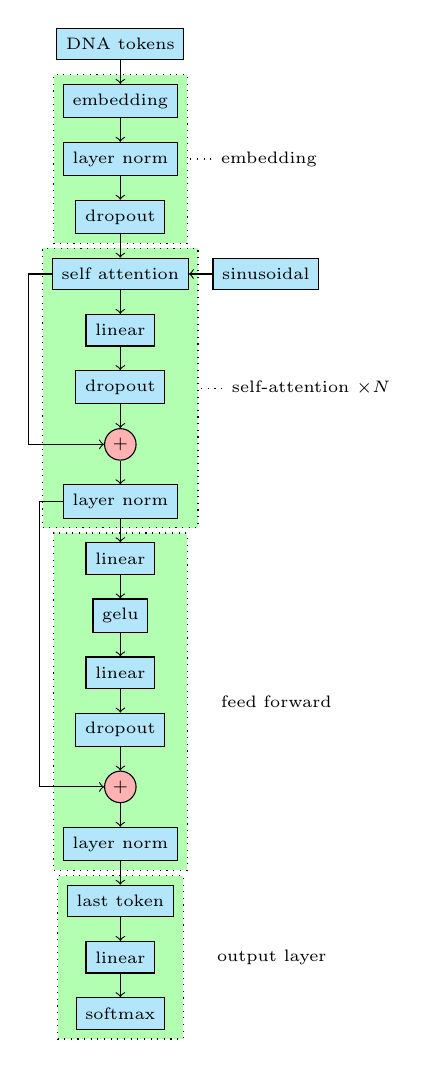
\begin{tikzpicture}
    \node[layer] (token) {DNA tokens};
    \node[layer, below=of token] (ebdEbd) {embedding};
    \node[layer, below=of ebdEbd] (ebdNorm) {layer norm};
    \node[layer, below=of ebdNorm] (ebdDrop) {dropout};
    \node[layer, below=of ebdDrop] (attAtt) {self attention};
    \node[layer, right=of attAtt] (sinusoidal) {sinusoidal};
    \node[layer, below=of attAtt] (attLinear) {linear};
    \node[layer, below=of attLinear] (attDrop) {dropout};
    \node[sum, below=of attDrop] (attSum) {+};
    \node[layer, below=of attSum] (attNorm) {layer norm};
    \node[layer, below=of attNorm] (ffnLinear) {linear};
    \node[layer, below=of ffnLinear] (ffnGelu) {gelu};
    \node[layer, below=of ffnGelu] (ffnLinear2) {linear};
    \node[layer, below=of ffnLinear2] (ffnDrop) {dropout};
    \node[sum, below=of ffnDrop] (ffnSum) {+};
    \node[layer, below=of ffnSum] (ffnNorm) {layer norm};
    \node[layer, below=of ffnNorm] (headLastToken) {last token};
    \node[layer, below=of headLastToken] (headLinear) {linear};
    \node[layer, below=of headLinear] (headSoftmax) {softmax};
    \graph {
      (token) -> (ebdEbd) -> (ebdNorm) -> (ebdDrop) -> (attAtt) -> (attLinear) -> (attDrop) -> (attSum) -> (attNorm) -> (ffnLinear) -> (ffnGelu) -> (ffnLinear2) -> (ffnDrop) -> (ffnSum) -> (ffnNorm) -> (headLastToken) -> (headLinear) -> (headSoftmax);
      (sinusoidal) -> (attAtt);
    };
    \draw[->] (attAtt) -- ($(attAtt.west) + (-3mm,0)$) |- (attSum);
    \draw[->] (attNorm) -- ($(attNorm.west) + (-3mm,0)$) |- (ffnSum);

    \begin{pgfonlayer}{background}
      \node[bkg, fit=(ebdEbd)(ebdNorm)(ebdDrop)](grpEbdMod) {};
      \node[annot, right=of grpEbdMod] (grpEbdModName) {embedding};
      \draw[dotted] (grpEbdModName) -- (grpEbdMod);
    \end{pgfonlayer}

    \begin{pgfonlayer}{background}
      \node[bkg, fit=(attAtt)(attLinear)(attDrop)(attSum)(attNorm)](grpAttMod) {};
      \node[annot, right=of grpAttMod] (grpAttModName) {self-attention $\times N$};
      \draw[dotted] (grpAttModName) -- (grpAttMod);
    \end{pgfonlayer}

    \begin{pgfonlayer}{background}
      \node[bkg, fit=(ffnLinear)(ffnGelu)(ffnLinear2)(ffnDrop)(ffnSum)(ffnNorm)] (grpFfnMod) {};
      \node[annot, right=of grpFfnMod] (grpFfnModName) {feed forward};
    \end{pgfonlayer}

    \begin{pgfonlayer}{background}
      \node[bkg, fit=(headLastToken)(headLinear)(headSoftmax)](grpHeadMod) {};
      \node[annot, right=of grpHeadMod] (grpHeadModName) {output layer};
    \end{pgfonlayer}
  \end{tikzpicture}
  \caption{CRIformer architecture in this paper.}\label{fig:criformer_architecture}
\end{figure}

\section{LSTM}

Resembling \cite{wang2019optimized}, we use the 21mer (protospacer + the first nucleotide of PAM) as the input to LSTM model. Besides the 21mer, we also provide some biological inputs to the model, including the free energy of the sgRNA + scaffold, the GC content of the protospacer, the melting temperatures of the whole 21mer input, the first four nucleotides, the middle eight nucleotides from the 5th to the 14th, and the last 5 nucleotides \cite{wang2019optimized}. As show in \cref{fig:lstm}, we embed the 21mer DNA sequence and apply channel-wise dropout. We then feed the result to the bidirectional LSTM layer and activates the output by tanh. We next concatenate the processed sequence input with the biological input and feed them to $N$ (in our case, 3) repeats of linear blocks composed of a linear layer, a elu activation and a dropout layer. Finally, we use an out linear layer to project the embedding space to the $32\times 32$ logits and use a softmax layer to transform the logits to the predicted editing profile.

\begin{figure}[H]
  \centering
  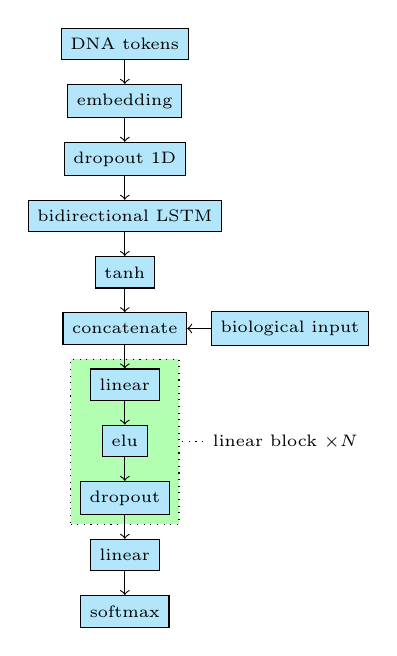
\begin{tikzpicture}
    \node[layer] (token) {DNA tokens};
    \node[layer, below=of token] (ebdEbd) {embedding};
    \node[layer, below=of ebdEbd] (drop1d) {dropout 1D};
    \node[layer, below=of drop1d] (biLSTM) {bidirectional LSTM};
    \node[layer, below=of biLSTM] (tanh) {tanh};
    \node[layer, below=of tanh] (cat) {concatenate};
    \node[layer, right=of cat] (bio) [] {biological input};
    \node[layer, below=of cat] (linear) {linear};
    \node[layer, below=of linear] (elu) {elu};
    \node[layer, below=of elu] (drop) {dropout};
    \node[layer, below=of drop] (outLinear) {linear};
    \node[layer, below=of outLinear] (softmax) {softmax};    
    \graph {
      (token) -> (ebdEbd) -> (drop1d) -> (biLSTM) -> (tanh) -> (cat) -> (linear) -> (elu) -> (drop) -> (outLinear) -> (softmax);
      (bio) -> (cat);
    };

    \begin{pgfonlayer}{background}
      \node[bkg, fit=(linear)(elu)(drop)](grpLinear) {};
      \node[annot, right=of grpLinear] (grpLinearName) {linear block $\times N$};
      \draw[dotted] (grpLinearName) -- (grpLinear);
    \end{pgfonlayer}
  \end{tikzpicture}
\caption{The LSTM architecture.}\label{fig:lstm}
\end{figure}

\section{CNN}

The CNN architecture is similar to the LSTM architecture. The difference is that the bidirectional LSTM becomes parallel CNN blocks. Also, we use the relu activation function to replace the elu in the LSTM architecture (see \cref{fig:CNN}).

\begin{figure}[H]
  \centering
  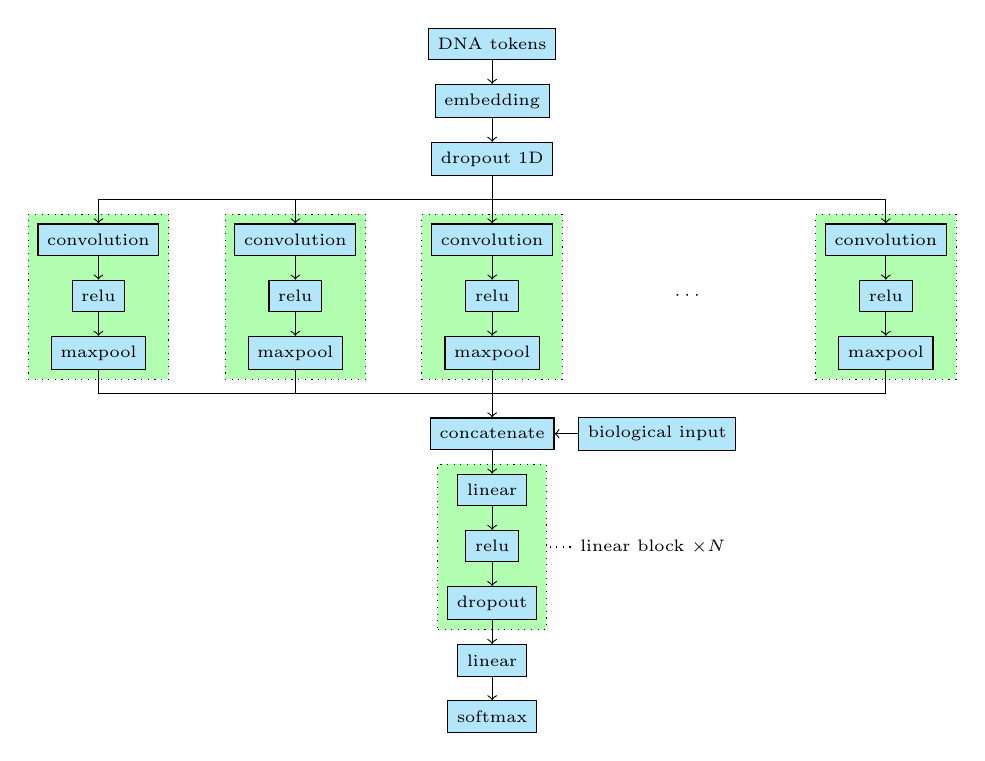
\begin{tikzpicture}
    \node[layer] (token) {DNA tokens};
    \node[layer, below=of token] (ebdEbd) {embedding};
    \node[layer, below=of ebdEbd] (drop1d) {dropout 1D};
    \coordinate[below=of drop1d] (conv2start);
    \begin{scope}[node distance=25mm]
      \coordinate[left=of conv2start] (conv1start);
      \coordinate[left=of conv1start] (conv0start);
      \coordinate[right=50mm of conv2start] (conv4start);
    \end{scope}
    \node[layer, below=of conv0start] (conv0) {convolution};
    \node[layer, below=of conv0] (conv0Relu) {relu};
    \node[layer, below=of conv0Relu] (conv0Maxpool) {maxpool};
    \coordinate[below=of conv0Maxpool] (conv0End);
    \node[layer, below=of conv1start] (conv1) {convolution};
    \node[layer, below=of conv1] (conv1Relu) {relu};
    \node[layer, below=of conv1Relu] (conv1Maxpool) {maxpool};
    \coordinate[below=of conv1Maxpool] (conv1End);
    \node[layer, below=of conv4start] (conv4) {convolution};
    \node[layer, below=of conv4] (conv4Relu) {relu};
    \node[layer, below=of conv4Relu] (conv4Maxpool) {maxpool};
    \coordinate[below=of conv4Maxpool] (conv4End);
    \node[layer, below=of conv2start] (conv2) {convolution};
    \node[layer, below=of conv2] (conv2Relu) {relu};
    \node[layer, below=of conv2Relu] (conv2Maxpool) {maxpool};
    \coordinate[below=of conv2Maxpool] (conv2End);
    \node[layer, below=of conv2End] (cat) {concatenate};
    \node[layer, right=of cat] (bio) {biological input};
    \node[layer, below=of cat] (linear) {linear};
    \node[layer, below=of linear] (relu) {relu};
    \node[layer, below=of relu] (drop) {dropout};
    \node[layer, below=of drop] (outLinear) {linear};
    \node[layer, below=of outLinear] (softmax) {softmax};
    \graph {
      (token) -> (ebdEbd) -> (drop1d) -- (conv2start) -> (conv2) -> (conv2Relu) -> (conv2Maxpool) -- (conv2End) -> (cat) -> (linear) -> (relu) -> (drop) -> (outLinear) -> (softmax);
      (bio) -> (cat);
      (conv1start) -- (conv0start) -> (conv0) -> (conv0Relu) -> (conv0Maxpool) -- (conv0End) -- (conv1End);
      (conv2start) -- (conv1start) -> (conv1) -> (conv1Relu) -> (conv1Maxpool) -- (conv1End) -- (conv2End);
      (conv2start) -- (conv4start) -> (conv4) -> (conv4Relu) -> (conv4Maxpool) -- (conv4End) -- (conv2End);
    };

    \begin{pgfonlayer}{background}
      \node[bkg, fit=(conv0)(conv0Relu)(conv0Maxpool)](grpLinear) {};
    \end{pgfonlayer}

    \begin{pgfonlayer}{background}
      \node[bkg, fit=(conv1)(conv1Relu)(conv1Maxpool)](grpLinear) {};
    \end{pgfonlayer}

    \begin{pgfonlayer}{background}
      \node[bkg, fit=(conv2)(conv2Relu)(conv2Maxpool)](grpLinear) {};
    \end{pgfonlayer}

    \begin{pgfonlayer}{background}
      \node[bkg, fit=(conv4)(conv4Relu)(conv4Maxpool)](grpLinear) {};
    \end{pgfonlayer}

    \path (conv2Relu) -- (conv4Relu) node[annot,midway] {$\cdots$};

    \begin{pgfonlayer}{background}
      \node[bkg, fit=(linear)(relu)(drop)](grpLinear) {};
      \node[annot, right=of grpLinear] (grpLinearName) {linear block $\times N$};
      \draw[dotted] (grpLinearName) -- (grpLinear);
    \end{pgfonlayer}
  \end{tikzpicture}
  \caption{The CNN architecture.}\label{fig:CNN}
\end{figure}

\section{MLP}

The MLP architecture represents the 21mer DNA as one-hot encoding, and concatenate it with the biological input. Then we simply repeats linear, sigmoid and dropout hidden layers for $N$-times (in our setting, 5 times). Finally, we use a linear layer to project the output of hidden layers to the $32\times 32$ logit tensor and transform it to the editing profile by the softmax layer.
\begin{figure}[H]
  \centering
  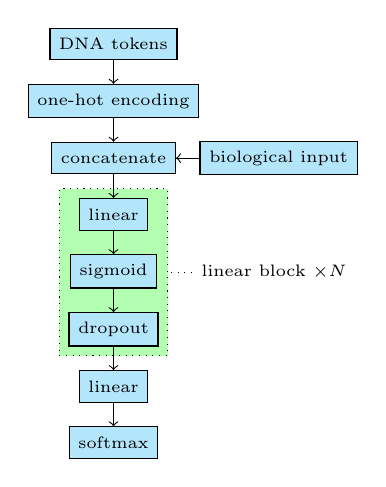
\begin{tikzpicture}
    \node[layer] (token) {DNA tokens};
    \node[layer, below=of token] (oneHot) {one-hot encoding};
    \node[layer, below=of oneHot] (cat) {concatenate};
    \node[layer, right=of cat] (bio) {biological input};
    \node[layer, below=of cat] (linear) {linear};
    \node[layer, below=of linear] (sigmoid) {sigmoid};
    \node[layer, below=of sigmoid] (drop) {dropout};
    \node[layer, below=of drop] (outLinear) {linear};
    \node[layer, below=of outLinear] (softmax) {softmax};
    \graph {
      (token) -> (oneHot) -> (cat) -> (linear) -> (sigmoid) -> (drop) -> (outLinear) -> (softmax);
      (bio) -> (cat);
    };

    \begin{pgfonlayer}{background}
      \node[bkg, fit=(linear)(sigmoid)(drop)](grpLinear) {};
      \node[annot, right=of grpLinear] (grpLinearName) {linear block $\times N$};
      \draw[dotted] (grpLinearName) -- (grpLinear);
    \end{pgfonlayer}
  \end{tikzpicture}
  \caption{The MLP architecture.}\label{fig:MLP}
\end{figure}

\bibliographystyle{plain}
\bibliography{reference.bib}

\end{document}